\section{Analysis of Formalization Quality}\label{sec:quality}
In our previous work,
we did not find metrics for detecting defects in software systems suitable to detect lints in formalizations~\cite{Formal2022Huch}.
However, the concept of code smells in software is more closely related to formalization code,
because the concept of code anti-patterns is transferable to formalizations.
In fact,
the Isabelle linter offers detection for a wide range of different anti-patterns~\cite{Linter2022Megdiche},
but not all of them are universally agreed on to have a detrimental effect on quality---%
for instance, some are specifically designed for certain styles.
With the editors of the AFP, we discussed which of the available lints should be executed on new submissions.
A few checks were suitable only for new submissions (e.g., the use of phased-out Isabelle commands),
and the following subset was agreed on to indicate actual quality problems
(even for existing material)\footnote{
Some of those criteria are checked by a combination of multiple lints.}:
\begin{enumerate}
%\\%apply_isar_switch
\item \emph{Switch between apply-style and Isar}
as such proofs are \enquote{hacked together} and not written down properly
(and hence hard to read).
%\\%counter_example_finder,proof_finder
\item \emph{Counter-example and proof-finder commands}
which are left over from interactive use,
and only affect the proof-checking speed in the archive.
%,diagnostic_command
\item \emph{Diagnostic commands} which are left over as well,
though sometimes intentionally for documentation purposes.
%\\%global_attribute_changes
\item \emph{Changes of global lemma attributes}
as such changes should only be made in a local context
so as not to affect users of the formalization.
%\\%global_attribute_on_unnamed_lemma
\item \emph{Unnamed lemmas in prover collections}
(e.g., the simplification set),
as without a name to address them, those lemmas can't be disabled.
%\\%unrestricted_auto,simplifier_isar_initial_method
\item \emph{Use of auto-style methods as non-terminal proofs methods},
which makes the following proof steps brittle as they rely on goals generated by aggressive rewriting.
\item \emph{Structured proof starting with an auto-style method} which is an especially bad version of the former,
as then the entire proof structure can change.
%\\%complex_method,complex_isar_initial_method
\item \emph{Overly complex methods}
as they make it very hard to read and follow a proof.
%\\%tactic_proofs
\item \emph{Tactic proofs}
since they allow to refer to system-generated names
which are arbitrary and could change at any point,
so they should not be explicitly referenced.
\end{enumerate}
These lints have been adopted in the AFP submission process and appear to be useful,
but there is no quantifiable proof of their effectiveness yet.

To account for file size,
we define \emph{lint frequency} to be the number of lints reported per line of Isabelle source code.
Hence, lint frequency is independent of file size.
To classify theories as good or problematic,
we use a pre-defined threshold of one lint per $100$ lines.
While this threshold is a bit arbitrary,
it seems appropriate given our previous experience with lints in Isabelle and the AFP,
where we found that one lint occurred every $200$ lines in HOL and four times more often in other sessions~\cite{Linter2022Megdiche}
(albeit with a different selection of lints).

Change-sets and churn can easily be measured for the Isabelle and AFP repositories\footnote{Merge commits are omitted as they only exist for technical reasons.}.
Of course, not all changes are due to maintenance problems---%
many authors contribute further additions and improvements
(e.g., better naming) to their developments.
We consider change-sets affecting more than a \emph{single} development to represent maintenance effort,
assuming that developers generate coherent change-sets that don't put the codebase into an inoperable state---%
under that assumption,
change-sets affecting \emph{multiple} developments correspond to changes that break other entries which then need to be repaired,
which is maintenance effort by definition.
It should be noted that maintenance effort is not necessarily caused by poor maintainability of a theory:
some edits induced by upstream changes might be unavoidable,
e.g., re-naming of a lemma that is later explicitly mentioned.
Still, change frequency should be a reasonable measure to approximate maintainability.

We quantify the above metrics over the Isabelle and AFP libraries to answer the following specific research questions:
\begin{enumerate}[label=\bfseries{RQ\arabic*}:, leftmargin=*]
\item Which of the problems uncovered by lints actually increase maintenance effort?
\item Are formalizations where many lints occur structurally different from others?
\item How much do lints reflect on perceived quality? Do other models?
\end{enumerate}

Our data are based on the Isabelle2022 release,
excluding tools as they are mostly not written in Isabelle/Isar
(and hence not covered by the Linter),
example theories since they could differ a lot from regular material,
and particularly slow developments due to computation time considerations.
A total of $6470$ theory files remain.
In the sections that follow we address each research question individually.

\subsection{Maintenance Effort}
Since we rely on the notion of single or multiple AFP developments for change frequencies,
we do not consider theories of the Isabelle distribution itself here,
leaving us $6160$ AFP theories.
On average, such a theory file is changed every $506$ days, and $139$ lines are edited in a change.
Figure~\ref{fig:changefreq_violin} shows violin plots for the distribution of change frequencies for change-sets affecting a single and multiple developments,
separated by whether lints occur frequently (i.e., more often than one lint every $100$ lines) in the theory.
\begin{figure}
\centering


% Created by tikzDevice version 0.12.4 on 2023-04-04 15:37:59
% !TEX encoding = UTF-8 Unicode
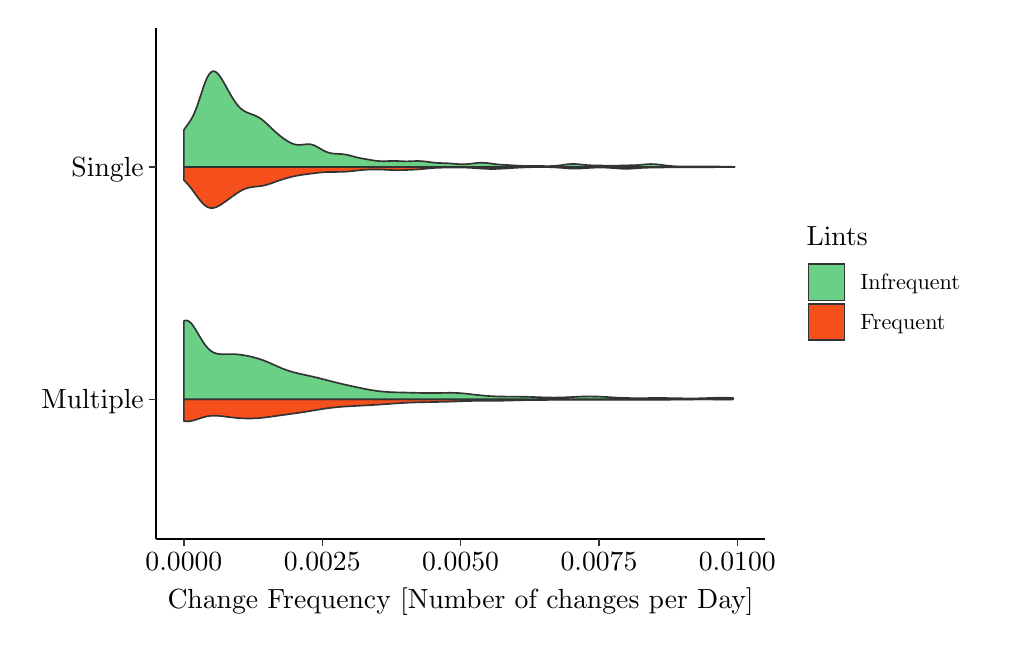
\begin{tikzpicture}[x=1pt,y=1pt]
\definecolor{plotBlue}{RGB}{77,126,255}
\definecolor{plotPurple}{RGB}{97,75,202}
\definecolor{plotViolet}{RGB}{199,42,119}
\definecolor{plotOrange}{RGB}{245,80,27}
\definecolor{plotGreen}{RGB}{105,208,134}
\definecolor{plotBlack}{RGB}{255,255,255}
\definecolor{fillColor}{RGB}{255,255,255}
\path[use as bounding box,fill=fillColor,fill opacity=0.00] (0,0) rectangle (346.90,216.81);
\begin{scope}
\path[clip] (  0.00,  0.00) rectangle (346.90,216.81);
\definecolor{drawColor}{RGB}{255,255,255}
\definecolor{fillColor}{RGB}{255,255,255}

\path[draw=drawColor,line width= 0.5pt,line join=round,line cap=round,fill=fillColor] ( -0.00,  0.00) rectangle (346.90,216.81);
\end{scope}
\begin{scope}
\path[clip] ( 46.44, 32.16) rectangle (266.43,216.81);
\definecolor{fillColor}{RGB}{255,255,255}

\path[fill=fillColor] ( 46.44, 32.16) rectangle (266.43,216.81);
\definecolor{drawColor}{gray}{0.20}

\path[draw=drawColor,line width= 0.6pt,line join=round,fill=plotOrange] ( 56.44, 82.52) --
	( 56.44, 74.69) --
	( 56.82, 74.62) --
	( 57.21, 74.57) --
	( 57.60, 74.55) --
	( 57.99, 74.56) --
	( 58.37, 74.59) --
	( 58.76, 74.64) --
	( 59.15, 74.71) --
	( 59.54, 74.79) --
	( 59.93, 74.89) --
	( 60.31, 75.00) --
	( 60.70, 75.12) --
	( 61.09, 75.25) --
	( 61.48, 75.38) --
	( 61.86, 75.51) --
	( 62.25, 75.64) --
	( 62.64, 75.77) --
	( 63.03, 75.89) --
	( 63.42, 76.01) --
	( 63.80, 76.11) --
	( 64.19, 76.21) --
	( 64.58, 76.30) --
	( 64.97, 76.38) --
	( 65.35, 76.44) --
	( 65.74, 76.49) --
	( 66.13, 76.54) --
	( 66.52, 76.57) --
	( 66.91, 76.59) --
	( 67.29, 76.59) --
	( 67.68, 76.59) --
	( 68.07, 76.59) --
	( 68.46, 76.57) --
	( 68.84, 76.54) --
	( 69.23, 76.51) --
	( 69.62, 76.48) --
	( 70.01, 76.44) --
	( 70.40, 76.40) --
	( 70.78, 76.35) --
	( 71.17, 76.30) --
	( 71.56, 76.25) --
	( 71.95, 76.20) --
	( 72.34, 76.15) --
	( 72.72, 76.11) --
	( 73.11, 76.06) --
	( 73.50, 76.01) --
	( 73.89, 75.96) --
	( 74.27, 75.92) --
	( 74.66, 75.88) --
	( 75.05, 75.84) --
	( 75.44, 75.80) --
	( 75.83, 75.77) --
	( 76.21, 75.74) --
	( 76.60, 75.71) --
	( 76.99, 75.68) --
	( 77.38, 75.66) --
	( 77.76, 75.64) --
	( 78.15, 75.63) --
	( 78.54, 75.61) --
	( 78.93, 75.60) --
	( 79.32, 75.59) --
	( 79.70, 75.59) --
	( 80.09, 75.59) --
	( 80.48, 75.59) --
	( 80.87, 75.60) --
	( 81.25, 75.61) --
	( 81.64, 75.62) --
	( 82.03, 75.64) --
	( 82.42, 75.66) --
	( 82.81, 75.68) --
	( 83.19, 75.71) --
	( 83.58, 75.74) --
	( 83.97, 75.77) --
	( 84.36, 75.81) --
	( 84.74, 75.85) --
	( 85.13, 75.89) --
	( 85.52, 75.94) --
	( 85.91, 75.98) --
	( 86.30, 76.03) --
	( 86.68, 76.08) --
	( 87.07, 76.13) --
	( 87.46, 76.18) --
	( 87.85, 76.24) --
	( 88.24, 76.29) --
	( 88.62, 76.35) --
	( 89.01, 76.40) --
	( 89.40, 76.46) --
	( 89.79, 76.51) --
	( 90.17, 76.57) --
	( 90.56, 76.62) --
	( 90.95, 76.68) --
	( 91.34, 76.73) --
	( 91.73, 76.79) --
	( 92.11, 76.84) --
	( 92.50, 76.89) --
	( 92.89, 76.94) --
	( 93.28, 77.00) --
	( 93.66, 77.05) --
	( 94.05, 77.10) --
	( 94.44, 77.15) --
	( 94.83, 77.20) --
	( 95.22, 77.25) --
	( 95.60, 77.31) --
	( 95.99, 77.36) --
	( 96.38, 77.41) --
	( 96.77, 77.47) --
	( 97.15, 77.52) --
	( 97.54, 77.58) --
	( 97.93, 77.63) --
	( 98.32, 77.69) --
	( 98.71, 77.75) --
	( 99.09, 77.81) --
	( 99.48, 77.87) --
	( 99.87, 77.93) --
	(100.26, 77.99) --
	(100.64, 78.05) --
	(101.03, 78.12) --
	(101.42, 78.18) --
	(101.81, 78.25) --
	(102.20, 78.31) --
	(102.58, 78.38) --
	(102.97, 78.44) --
	(103.36, 78.51) --
	(103.75, 78.57) --
	(104.14, 78.64) --
	(104.52, 78.70) --
	(104.91, 78.77) --
	(105.30, 78.83) --
	(105.69, 78.89) --
	(106.07, 78.95) --
	(106.46, 79.01) --
	(106.85, 79.07) --
	(107.24, 79.13) --
	(107.63, 79.19) --
	(108.01, 79.24) --
	(108.40, 79.29) --
	(108.79, 79.34) --
	(109.18, 79.39) --
	(109.56, 79.44) --
	(109.95, 79.48) --
	(110.34, 79.53) --
	(110.73, 79.57) --
	(111.12, 79.61) --
	(111.50, 79.65) --
	(111.89, 79.69) --
	(112.28, 79.72) --
	(112.67, 79.75) --
	(113.05, 79.79) --
	(113.44, 79.82) --
	(113.83, 79.85) --
	(114.22, 79.87) --
	(114.61, 79.90) --
	(114.99, 79.93) --
	(115.38, 79.95) --
	(115.77, 79.97) --
	(116.16, 80.00) --
	(116.54, 80.02) --
	(116.93, 80.04) --
	(117.32, 80.06) --
	(117.71, 80.09) --
	(118.10, 80.11) --
	(118.48, 80.13) --
	(118.87, 80.15) --
	(119.26, 80.17) --
	(119.65, 80.19) --
	(120.04, 80.21) --
	(120.42, 80.23) --
	(120.81, 80.25) --
	(121.20, 80.27) --
	(121.59, 80.29) --
	(121.97, 80.31) --
	(122.36, 80.33) --
	(122.75, 80.35) --
	(123.14, 80.38) --
	(123.53, 80.40) --
	(123.91, 80.42) --
	(124.30, 80.44) --
	(124.69, 80.47) --
	(125.08, 80.49) --
	(125.46, 80.51) --
	(125.85, 80.54) --
	(126.24, 80.56) --
	(126.63, 80.59) --
	(127.02, 80.61) --
	(127.40, 80.64) --
	(127.79, 80.67) --
	(128.18, 80.69) --
	(128.57, 80.72) --
	(128.95, 80.75) --
	(129.34, 80.77) --
	(129.73, 80.80) --
	(130.12, 80.83) --
	(130.51, 80.85) --
	(130.89, 80.88) --
	(131.28, 80.91) --
	(131.67, 80.94) --
	(132.06, 80.96) --
	(132.44, 80.99) --
	(132.83, 81.02) --
	(133.22, 81.05) --
	(133.61, 81.07) --
	(134.00, 81.10) --
	(134.38, 81.12) --
	(134.77, 81.15) --
	(135.16, 81.17) --
	(135.55, 81.19) --
	(135.94, 81.22) --
	(136.32, 81.24) --
	(136.71, 81.26) --
	(137.10, 81.28) --
	(137.49, 81.30) --
	(137.87, 81.32) --
	(138.26, 81.33) --
	(138.65, 81.35) --
	(139.04, 81.36) --
	(139.43, 81.38) --
	(139.81, 81.39) --
	(140.20, 81.40) --
	(140.59, 81.41) --
	(140.98, 81.42) --
	(141.36, 81.43) --
	(141.75, 81.44) --
	(142.14, 81.45) --
	(142.53, 81.46) --
	(142.92, 81.47) --
	(143.30, 81.48) --
	(143.69, 81.48) --
	(144.08, 81.49) --
	(144.47, 81.50) --
	(144.85, 81.51) --
	(145.24, 81.51) --
	(145.63, 81.52) --
	(146.02, 81.53) --
	(146.41, 81.54) --
	(146.79, 81.54) --
	(147.18, 81.55) --
	(147.57, 81.56) --
	(147.96, 81.57) --
	(148.34, 81.57) --
	(148.73, 81.58) --
	(149.12, 81.59) --
	(149.51, 81.60) --
	(149.90, 81.61) --
	(150.28, 81.62) --
	(150.67, 81.62) --
	(151.06, 81.63) --
	(151.45, 81.64) --
	(151.84, 81.65) --
	(152.22, 81.67) --
	(152.61, 81.68) --
	(153.00, 81.69) --
	(153.39, 81.70) --
	(153.77, 81.71) --
	(154.16, 81.72) --
	(154.55, 81.74) --
	(154.94, 81.75) --
	(155.33, 81.76) --
	(155.71, 81.78) --
	(156.10, 81.79) --
	(156.49, 81.81) --
	(156.88, 81.82) --
	(157.26, 81.83) --
	(157.65, 81.85) --
	(158.04, 81.86) --
	(158.43, 81.87) --
	(158.82, 81.88) --
	(159.20, 81.90) --
	(159.59, 81.91) --
	(159.98, 81.92) --
	(160.37, 81.93) --
	(160.75, 81.94) --
	(161.14, 81.94) --
	(161.53, 81.95) --
	(161.92, 81.96) --
	(162.31, 81.96) --
	(162.69, 81.97) --
	(163.08, 81.97) --
	(163.47, 81.97) --
	(163.86, 81.98) --
	(164.24, 81.98) --
	(164.63, 81.98) --
	(165.02, 81.98) --
	(165.41, 81.98) --
	(165.80, 81.98) --
	(166.18, 81.98) --
	(166.57, 81.98) --
	(166.96, 81.98) --
	(167.35, 81.98) --
	(167.74, 81.98) --
	(168.12, 81.98) --
	(168.51, 81.98) --
	(168.90, 81.98) --
	(169.29, 81.99) --
	(169.67, 81.99) --
	(170.06, 81.99) --
	(170.45, 82.00) --
	(170.84, 82.00) --
	(171.23, 82.01) --
	(171.61, 82.02) --
	(172.00, 82.03) --
	(172.39, 82.04) --
	(172.78, 82.04) --
	(173.16, 82.05) --
	(173.55, 82.07) --
	(173.94, 82.08) --
	(174.33, 82.09) --
	(174.72, 82.10) --
	(175.10, 82.11) --
	(175.49, 82.12) --
	(175.88, 82.13) --
	(176.27, 82.15) --
	(176.65, 82.16) --
	(177.04, 82.17) --
	(177.43, 82.18) --
	(177.82, 82.19) --
	(178.21, 82.20) --
	(178.59, 82.21) --
	(178.98, 82.22) --
	(179.37, 82.23) --
	(179.76, 82.23) --
	(180.14, 82.24) --
	(180.53, 82.25) --
	(180.92, 82.25) --
	(181.31, 82.26) --
	(181.70, 82.26) --
	(182.08, 82.27) --
	(182.47, 82.27) --
	(182.86, 82.27) --
	(183.25, 82.28) --
	(183.64, 82.28) --
	(184.02, 82.28) --
	(184.41, 82.28) --
	(184.80, 82.29) --
	(185.19, 82.29) --
	(185.57, 82.29) --
	(185.96, 82.29) --
	(186.35, 82.29) --
	(186.74, 82.29) --
	(187.13, 82.29) --
	(187.51, 82.29) --
	(187.90, 82.30) --
	(188.29, 82.30) --
	(188.68, 82.30) --
	(189.06, 82.30) --
	(189.45, 82.30) --
	(189.84, 82.30) --
	(190.23, 82.31) --
	(190.62, 82.31) --
	(191.00, 82.31) --
	(191.39, 82.31) --
	(191.78, 82.32) --
	(192.17, 82.32) --
	(192.55, 82.32) --
	(192.94, 82.33) --
	(193.33, 82.33) --
	(193.72, 82.33) --
	(194.11, 82.34) --
	(194.49, 82.34) --
	(194.88, 82.34) --
	(195.27, 82.35) --
	(195.66, 82.35) --
	(196.04, 82.35) --
	(196.43, 82.36) --
	(196.82, 82.36) --
	(197.21, 82.36) --
	(197.60, 82.37) --
	(197.98, 82.37) --
	(198.37, 82.37) --
	(198.76, 82.37) --
	(199.15, 82.37) --
	(199.54, 82.37) --
	(199.92, 82.37) --
	(200.31, 82.37) --
	(200.70, 82.37) --
	(201.09, 82.37) --
	(201.47, 82.37) --
	(201.86, 82.36) --
	(202.25, 82.36) --
	(202.64, 82.36) --
	(203.03, 82.36) --
	(203.41, 82.35) --
	(203.80, 82.35) --
	(204.19, 82.35) --
	(204.58, 82.34) --
	(204.96, 82.34) --
	(205.35, 82.34) --
	(205.74, 82.33) --
	(206.13, 82.33) --
	(206.52, 82.33) --
	(206.90, 82.32) --
	(207.29, 82.32) --
	(207.68, 82.32) --
	(208.07, 82.31) --
	(208.45, 82.31) --
	(208.84, 82.31) --
	(209.23, 82.31) --
	(209.62, 82.31) --
	(210.01, 82.30) --
	(210.39, 82.30) --
	(210.78, 82.30) --
	(211.17, 82.30) --
	(211.56, 82.30) --
	(211.94, 82.30) --
	(212.33, 82.30) --
	(212.72, 82.30) --
	(213.11, 82.30) --
	(213.50, 82.30) --
	(213.88, 82.30) --
	(214.27, 82.30) --
	(214.66, 82.30) --
	(215.05, 82.30) --
	(215.44, 82.30) --
	(215.82, 82.30) --
	(216.21, 82.30) --
	(216.60, 82.30) --
	(216.99, 82.30) --
	(217.37, 82.30) --
	(217.76, 82.30) --
	(218.15, 82.30) --
	(218.54, 82.30) --
	(218.93, 82.30) --
	(219.31, 82.30) --
	(219.70, 82.30) --
	(220.09, 82.30) --
	(220.48, 82.30) --
	(220.86, 82.30) --
	(221.25, 82.30) --
	(221.64, 82.30) --
	(222.03, 82.30) --
	(222.42, 82.30) --
	(222.80, 82.30) --
	(223.19, 82.30) --
	(223.58, 82.30) --
	(223.97, 82.30) --
	(224.35, 82.30) --
	(224.74, 82.30) --
	(225.13, 82.30) --
	(225.52, 82.30) --
	(225.91, 82.31) --
	(226.29, 82.31) --
	(226.68, 82.31) --
	(227.07, 82.32) --
	(227.46, 82.32) --
	(227.84, 82.32) --
	(228.23, 82.33) --
	(228.62, 82.33) --
	(229.01, 82.34) --
	(229.40, 82.34) --
	(229.78, 82.35) --
	(230.17, 82.35) --
	(230.56, 82.36) --
	(230.95, 82.37) --
	(231.34, 82.37) --
	(231.72, 82.38) --
	(232.11, 82.38) --
	(232.50, 82.39) --
	(232.89, 82.40) --
	(233.27, 82.40) --
	(233.66, 82.41) --
	(234.05, 82.41) --
	(234.44, 82.42) --
	(234.83, 82.42) --
	(235.21, 82.43) --
	(235.60, 82.43) --
	(235.99, 82.44) --
	(236.38, 82.44) --
	(236.76, 82.45) --
	(237.15, 82.45) --
	(237.54, 82.45) --
	(237.93, 82.46) --
	(238.32, 82.46) --
	(238.70, 82.46) --
	(239.09, 82.47) --
	(239.48, 82.47) --
	(239.87, 82.47) --
	(240.25, 82.47) --
	(240.64, 82.48) --
	(241.03, 82.48) --
	(241.42, 82.48) --
	(241.81, 82.48) --
	(242.19, 82.48) --
	(242.58, 82.48) --
	(242.97, 82.48) --
	(243.36, 82.48) --
	(243.74, 82.48) --
	(244.13, 82.48) --
	(244.52, 82.48) --
	(244.91, 82.48) --
	(245.30, 82.48) --
	(245.68, 82.48) --
	(246.07, 82.48) --
	(246.46, 82.48) --
	(246.85, 82.48) --
	(247.24, 82.48) --
	(247.62, 82.48) --
	(248.01, 82.47) --
	(248.40, 82.47) --
	(248.79, 82.47) --
	(249.17, 82.47) --
	(249.56, 82.47) --
	(249.95, 82.47) --
	(250.34, 82.47) --
	(250.73, 82.47) --
	(251.11, 82.47) --
	(251.50, 82.47) --
	(251.89, 82.47) --
	(252.28, 82.47) --
	(252.66, 82.47) --
	(253.05, 82.47) --
	(253.44, 82.47) --
	(253.83, 82.47) --
	(254.22, 82.47) --
	(254.60, 82.47) --
	(254.60, 82.52) --
	( 56.44, 82.52) --
	cycle;

\path[draw=drawColor,line width= 0.6pt,line join=round,fill=plotGreen] (254.93, 82.52) --
	(254.93, 82.97) --
	(254.54, 82.99) --
	(254.15, 83.01) --
	(253.76, 83.02) --
	(253.37, 83.04) --
	(252.98, 83.05) --
	(252.59, 83.06) --
	(252.21, 83.07) --
	(251.82, 83.08) --
	(251.43, 83.08) --
	(251.04, 83.08) --
	(250.65, 83.09) --
	(250.26, 83.09) --
	(249.88, 83.08) --
	(249.49, 83.08) --
	(249.10, 83.07) --
	(248.71, 83.06) --
	(248.32, 83.05) --
	(247.93, 83.04) --
	(247.54, 83.03) --
	(247.16, 83.02) --
	(246.77, 83.01) --
	(246.38, 82.99) --
	(245.99, 82.98) --
	(245.60, 82.97) --
	(245.21, 82.95) --
	(244.83, 82.94) --
	(244.44, 82.93) --
	(244.05, 82.91) --
	(243.66, 82.90) --
	(243.27, 82.89) --
	(242.88, 82.88) --
	(242.50, 82.87) --
	(242.11, 82.86) --
	(241.72, 82.86) --
	(241.33, 82.85) --
	(240.94, 82.85) --
	(240.55, 82.85) --
	(240.16, 82.84) --
	(239.78, 82.84) --
	(239.39, 82.84) --
	(239.00, 82.84) --
	(238.61, 82.85) --
	(238.22, 82.85) --
	(237.83, 82.85) --
	(237.45, 82.86) --
	(237.06, 82.86) --
	(236.67, 82.87) --
	(236.28, 82.88) --
	(235.89, 82.88) --
	(235.50, 82.89) --
	(235.11, 82.90) --
	(234.73, 82.91) --
	(234.34, 82.91) --
	(233.95, 82.92) --
	(233.56, 82.93) --
	(233.17, 82.93) --
	(232.78, 82.94) --
	(232.40, 82.95) --
	(232.01, 82.95) --
	(231.62, 82.96) --
	(231.23, 82.96) --
	(230.84, 82.97) --
	(230.45, 82.97) --
	(230.07, 82.97) --
	(229.68, 82.98) --
	(229.29, 82.98) --
	(228.90, 82.98) --
	(228.51, 82.98) --
	(228.12, 82.98) --
	(227.73, 82.98) --
	(227.35, 82.98) --
	(226.96, 82.98) --
	(226.57, 82.98) --
	(226.18, 82.98) --
	(225.79, 82.97) --
	(225.40, 82.97) --
	(225.02, 82.97) --
	(224.63, 82.97) --
	(224.24, 82.96) --
	(223.85, 82.96) --
	(223.46, 82.96) --
	(223.07, 82.96) --
	(222.68, 82.95) --
	(222.30, 82.95) --
	(221.91, 82.95) --
	(221.52, 82.95) --
	(221.13, 82.94) --
	(220.74, 82.94) --
	(220.35, 82.94) --
	(219.97, 82.94) --
	(219.58, 82.94) --
	(219.19, 82.94) --
	(218.80, 82.95) --
	(218.41, 82.95) --
	(218.02, 82.95) --
	(217.64, 82.96) --
	(217.25, 82.97) --
	(216.86, 82.98) --
	(216.47, 82.98) --
	(216.08, 82.99) --
	(215.69, 83.01) --
	(215.30, 83.02) --
	(214.92, 83.03) --
	(214.53, 83.05) --
	(214.14, 83.07) --
	(213.75, 83.08) --
	(213.36, 83.10) --
	(212.97, 83.12) --
	(212.59, 83.14) --
	(212.20, 83.16) --
	(211.81, 83.19) --
	(211.42, 83.21) --
	(211.03, 83.23) --
	(210.64, 83.26) --
	(210.26, 83.28) --
	(209.87, 83.31) --
	(209.48, 83.33) --
	(209.09, 83.35) --
	(208.70, 83.38) --
	(208.31, 83.40) --
	(207.92, 83.42) --
	(207.54, 83.44) --
	(207.15, 83.46) --
	(206.76, 83.48) --
	(206.37, 83.50) --
	(205.98, 83.51) --
	(205.59, 83.53) --
	(205.21, 83.54) --
	(204.82, 83.55) --
	(204.43, 83.56) --
	(204.04, 83.56) --
	(203.65, 83.57) --
	(203.26, 83.57) --
	(202.87, 83.57) --
	(202.49, 83.56) --
	(202.10, 83.56) --
	(201.71, 83.55) --
	(201.32, 83.54) --
	(200.93, 83.53) --
	(200.54, 83.52) --
	(200.16, 83.51) --
	(199.77, 83.49) --
	(199.38, 83.47) --
	(198.99, 83.46) --
	(198.60, 83.44) --
	(198.21, 83.42) --
	(197.83, 83.40) --
	(197.44, 83.38) --
	(197.05, 83.36) --
	(196.66, 83.34) --
	(196.27, 83.32) --
	(195.88, 83.30) --
	(195.49, 83.28) --
	(195.11, 83.27) --
	(194.72, 83.25) --
	(194.33, 83.23) --
	(193.94, 83.22) --
	(193.55, 83.20) --
	(193.16, 83.19) --
	(192.78, 83.18) --
	(192.39, 83.17) --
	(192.00, 83.16) --
	(191.61, 83.16) --
	(191.22, 83.15) --
	(190.83, 83.15) --
	(190.44, 83.14) --
	(190.06, 83.14) --
	(189.67, 83.14) --
	(189.28, 83.15) --
	(188.89, 83.15) --
	(188.50, 83.16) --
	(188.11, 83.16) --
	(187.73, 83.17) --
	(187.34, 83.18) --
	(186.95, 83.19) --
	(186.56, 83.20) --
	(186.17, 83.22) --
	(185.78, 83.23) --
	(185.40, 83.24) --
	(185.01, 83.26) --
	(184.62, 83.27) --
	(184.23, 83.29) --
	(183.84, 83.30) --
	(183.45, 83.32) --
	(183.06, 83.33) --
	(182.68, 83.35) --
	(182.29, 83.36) --
	(181.90, 83.38) --
	(181.51, 83.39) --
	(181.12, 83.40) --
	(180.73, 83.41) --
	(180.35, 83.43) --
	(179.96, 83.44) --
	(179.57, 83.44) --
	(179.18, 83.45) --
	(178.79, 83.46) --
	(178.40, 83.47) --
	(178.02, 83.47) --
	(177.63, 83.48) --
	(177.24, 83.48) --
	(176.85, 83.48) --
	(176.46, 83.49) --
	(176.07, 83.49) --
	(175.68, 83.49) --
	(175.30, 83.49) --
	(174.91, 83.49) --
	(174.52, 83.49) --
	(174.13, 83.49) --
	(173.74, 83.50) --
	(173.35, 83.50) --
	(172.97, 83.50) --
	(172.58, 83.50) --
	(172.19, 83.51) --
	(171.80, 83.51) --
	(171.41, 83.52) --
	(171.02, 83.53) --
	(170.63, 83.54) --
	(170.25, 83.55) --
	(169.86, 83.56) --
	(169.47, 83.57) --
	(169.08, 83.59) --
	(168.69, 83.60) --
	(168.30, 83.62) --
	(167.92, 83.64) --
	(167.53, 83.66) --
	(167.14, 83.68) --
	(166.75, 83.71) --
	(166.36, 83.73) --
	(165.97, 83.76) --
	(165.59, 83.79) --
	(165.20, 83.82) --
	(164.81, 83.86) --
	(164.42, 83.89) --
	(164.03, 83.93) --
	(163.64, 83.97) --
	(163.25, 84.01) --
	(162.87, 84.05) --
	(162.48, 84.09) --
	(162.09, 84.14) --
	(161.70, 84.18) --
	(161.31, 84.22) --
	(160.92, 84.27) --
	(160.54, 84.31) --
	(160.15, 84.36) --
	(159.76, 84.40) --
	(159.37, 84.45) --
	(158.98, 84.49) --
	(158.59, 84.53) --
	(158.20, 84.57) --
	(157.82, 84.61) --
	(157.43, 84.65) --
	(157.04, 84.68) --
	(156.65, 84.71) --
	(156.26, 84.74) --
	(155.87, 84.77) --
	(155.49, 84.79) --
	(155.10, 84.81) --
	(154.71, 84.82) --
	(154.32, 84.84) --
	(153.93, 84.85) --
	(153.54, 84.86) --
	(153.16, 84.86) --
	(152.77, 84.86) --
	(152.38, 84.86) --
	(151.99, 84.86) --
	(151.60, 84.86) --
	(151.21, 84.85) --
	(150.82, 84.85) --
	(150.44, 84.84) --
	(150.05, 84.83) --
	(149.66, 84.83) --
	(149.27, 84.82) --
	(148.88, 84.81) --
	(148.49, 84.81) --
	(148.11, 84.80) --
	(147.72, 84.79) --
	(147.33, 84.79) --
	(146.94, 84.79) --
	(146.55, 84.78) --
	(146.16, 84.78) --
	(145.77, 84.78) --
	(145.39, 84.78) --
	(145.00, 84.78) --
	(144.61, 84.79) --
	(144.22, 84.79) --
	(143.83, 84.79) --
	(143.44, 84.80) --
	(143.06, 84.81) --
	(142.67, 84.81) --
	(142.28, 84.82) --
	(141.89, 84.83) --
	(141.50, 84.84) --
	(141.11, 84.85) --
	(140.73, 84.85) --
	(140.34, 84.86) --
	(139.95, 84.87) --
	(139.56, 84.88) --
	(139.17, 84.89) --
	(138.78, 84.90) --
	(138.39, 84.91) --
	(138.01, 84.92) --
	(137.62, 84.93) --
	(137.23, 84.94) --
	(136.84, 84.95) --
	(136.45, 84.95) --
	(136.06, 84.96) --
	(135.68, 84.97) --
	(135.29, 84.98) --
	(134.90, 84.99) --
	(134.51, 85.00) --
	(134.12, 85.01) --
	(133.73, 85.02) --
	(133.35, 85.03) --
	(132.96, 85.04) --
	(132.57, 85.06) --
	(132.18, 85.07) --
	(131.79, 85.09) --
	(131.40, 85.10) --
	(131.01, 85.12) --
	(130.63, 85.14) --
	(130.24, 85.17) --
	(129.85, 85.19) --
	(129.46, 85.22) --
	(129.07, 85.25) --
	(128.68, 85.28) --
	(128.30, 85.32) --
	(127.91, 85.35) --
	(127.52, 85.39) --
	(127.13, 85.44) --
	(126.74, 85.48) --
	(126.35, 85.53) --
	(125.96, 85.58) --
	(125.58, 85.64) --
	(125.19, 85.70) --
	(124.80, 85.76) --
	(124.41, 85.82) --
	(124.02, 85.88) --
	(123.63, 85.95) --
	(123.25, 86.02) --
	(122.86, 86.09) --
	(122.47, 86.16) --
	(122.08, 86.24) --
	(121.69, 86.31) --
	(121.30, 86.39) --
	(120.92, 86.47) --
	(120.53, 86.55) --
	(120.14, 86.63) --
	(119.75, 86.71) --
	(119.36, 86.80) --
	(118.97, 86.88) --
	(118.58, 86.96) --
	(118.20, 87.05) --
	(117.81, 87.13) --
	(117.42, 87.21) --
	(117.03, 87.30) --
	(116.64, 87.38) --
	(116.25, 87.47) --
	(115.87, 87.56) --
	(115.48, 87.64) --
	(115.09, 87.73) --
	(114.70, 87.82) --
	(114.31, 87.90) --
	(113.92, 87.99) --
	(113.53, 88.08) --
	(113.15, 88.17) --
	(112.76, 88.26) --
	(112.37, 88.36) --
	(111.98, 88.45) --
	(111.59, 88.54) --
	(111.20, 88.64) --
	(110.82, 88.74) --
	(110.43, 88.83) --
	(110.04, 88.93) --
	(109.65, 89.03) --
	(109.26, 89.13) --
	(108.87, 89.23) --
	(108.49, 89.33) --
	(108.10, 89.43) --
	(107.71, 89.53) --
	(107.32, 89.64) --
	(106.93, 89.74) --
	(106.54, 89.84) --
	(106.15, 89.94) --
	(105.77, 90.03) --
	(105.38, 90.13) --
	(104.99, 90.23) --
	(104.60, 90.33) --
	(104.21, 90.42) --
	(103.82, 90.51) --
	(103.44, 90.60) --
	(103.05, 90.70) --
	(102.66, 90.79) --
	(102.27, 90.87) --
	(101.88, 90.96) --
	(101.49, 91.05) --
	(101.11, 91.13) --
	(100.72, 91.22) --
	(100.33, 91.30) --
	( 99.94, 91.39) --
	( 99.55, 91.47) --
	( 99.16, 91.56) --
	( 98.77, 91.64) --
	( 98.39, 91.73) --
	( 98.00, 91.82) --
	( 97.61, 91.91) --
	( 97.22, 92.01) --
	( 96.83, 92.10) --
	( 96.44, 92.20) --
	( 96.06, 92.30) --
	( 95.67, 92.41) --
	( 95.28, 92.52) --
	( 94.89, 92.64) --
	( 94.50, 92.76) --
	( 94.11, 92.89) --
	( 93.72, 93.02) --
	( 93.34, 93.16) --
	( 92.95, 93.30) --
	( 92.56, 93.45) --
	( 92.17, 93.60) --
	( 91.78, 93.75) --
	( 91.39, 93.91) --
	( 91.01, 94.08) --
	( 90.62, 94.25) --
	( 90.23, 94.42) --
	( 89.84, 94.59) --
	( 89.45, 94.77) --
	( 89.06, 94.94) --
	( 88.68, 95.12) --
	( 88.29, 95.29) --
	( 87.90, 95.46) --
	( 87.51, 95.64) --
	( 87.12, 95.80) --
	( 86.73, 95.97) --
	( 86.34, 96.13) --
	( 85.96, 96.29) --
	( 85.57, 96.44) --
	( 85.18, 96.59) --
	( 84.79, 96.73) --
	( 84.40, 96.86) --
	( 84.01, 97.00) --
	( 83.63, 97.12) --
	( 83.24, 97.24) --
	( 82.85, 97.36) --
	( 82.46, 97.47) --
	( 82.07, 97.58) --
	( 81.68, 97.68) --
	( 81.29, 97.78) --
	( 80.91, 97.87) --
	( 80.52, 97.96) --
	( 80.13, 98.05) --
	( 79.74, 98.13) --
	( 79.35, 98.21) --
	( 78.96, 98.29) --
	( 78.58, 98.36) --
	( 78.19, 98.43) --
	( 77.80, 98.49) --
	( 77.41, 98.55) --
	( 77.02, 98.61) --
	( 76.63, 98.66) --
	( 76.25, 98.70) --
	( 75.86, 98.74) --
	( 75.47, 98.78) --
	( 75.08, 98.81) --
	( 74.69, 98.83) --
	( 74.30, 98.84) --
	( 73.91, 98.86) --
	( 73.53, 98.86) --
	( 73.14, 98.86) --
	( 72.75, 98.86) --
	( 72.36, 98.85) --
	( 71.97, 98.84) --
	( 71.58, 98.83) --
	( 71.20, 98.82) --
	( 70.81, 98.81) --
	( 70.42, 98.81) --
	( 70.03, 98.82) --
	( 69.64, 98.84) --
	( 69.25, 98.87) --
	( 68.87, 98.93) --
	( 68.48, 99.00) --
	( 68.09, 99.09) --
	( 67.70, 99.22) --
	( 67.31, 99.38) --
	( 66.92, 99.57) --
	( 66.53, 99.80) --
	( 66.15,100.07) --
	( 65.76,100.38) --
	( 65.37,100.74) --
	( 64.98,101.15) --
	( 64.59,101.59) --
	( 64.20,102.08) --
	( 63.82,102.61) --
	( 63.43,103.18) --
	( 63.04,103.78) --
	( 62.65,104.41) --
	( 62.26,105.06) --
	( 61.87,105.72) --
	( 61.48,106.39) --
	( 61.10,107.05) --
	( 60.71,107.69) --
	( 60.32,108.31) --
	( 59.93,108.89) --
	( 59.54,109.43) --
	( 59.15,109.90) --
	( 58.77,110.29) --
	( 58.38,110.61) --
	( 57.99,110.85) --
	( 57.60,111.00) --
	( 57.21,111.04) --
	( 56.82,110.96) --
	( 56.44,110.78) --
	( 56.44, 82.52) --
	(254.93, 82.52) --
	cycle;

\path[draw=drawColor,line width= 0.6pt,line join=round,fill=plotOrange] ( 56.44,166.45) --
	( 56.44,161.75) --
	( 56.82,161.36) --
	( 57.21,160.95) --
	( 57.60,160.52) --
	( 57.99,160.08) --
	( 58.38,159.61) --
	( 58.77,159.13) --
	( 59.16,158.63) --
	( 59.55,158.11) --
	( 59.94,157.59) --
	( 60.33,157.05) --
	( 60.72,156.52) --
	( 61.11,155.98) --
	( 61.50,155.45) --
	( 61.89,154.94) --
	( 62.28,154.45) --
	( 62.67,153.98) --
	( 63.06,153.54) --
	( 63.44,153.14) --
	( 63.83,152.78) --
	( 64.22,152.46) --
	( 64.61,152.19) --
	( 65.00,151.98) --
	( 65.39,151.82) --
	( 65.78,151.71) --
	( 66.17,151.64) --
	( 66.56,151.63) --
	( 66.95,151.65) --
	( 67.34,151.72) --
	( 67.73,151.83) --
	( 68.12,151.97) --
	( 68.51,152.14) --
	( 68.90,152.34) --
	( 69.29,152.56) --
	( 69.68,152.79) --
	( 70.07,153.04) --
	( 70.45,153.30) --
	( 70.84,153.56) --
	( 71.23,153.84) --
	( 71.62,154.11) --
	( 72.01,154.40) --
	( 72.40,154.68) --
	( 72.79,154.96) --
	( 73.18,155.25) --
	( 73.57,155.53) --
	( 73.96,155.82) --
	( 74.35,156.10) --
	( 74.74,156.37) --
	( 75.13,156.64) --
	( 75.52,156.91) --
	( 75.91,157.16) --
	( 76.30,157.41) --
	( 76.69,157.64) --
	( 77.07,157.86) --
	( 77.46,158.07) --
	( 77.85,158.26) --
	( 78.24,158.43) --
	( 78.63,158.59) --
	( 79.02,158.73) --
	( 79.41,158.85) --
	( 79.80,158.96) --
	( 80.19,159.05) --
	( 80.58,159.12) --
	( 80.97,159.19) --
	( 81.36,159.24) --
	( 81.75,159.29) --
	( 82.14,159.33) --
	( 82.53,159.38) --
	( 82.92,159.42) --
	( 83.31,159.46) --
	( 83.70,159.51) --
	( 84.08,159.56) --
	( 84.47,159.62) --
	( 84.86,159.68) --
	( 85.25,159.76) --
	( 85.64,159.85) --
	( 86.03,159.95) --
	( 86.42,160.05) --
	( 86.81,160.16) --
	( 87.20,160.29) --
	( 87.59,160.41) --
	( 87.98,160.55) --
	( 88.37,160.69) --
	( 88.76,160.83) --
	( 89.15,160.97) --
	( 89.54,161.11) --
	( 89.93,161.26) --
	( 90.32,161.40) --
	( 90.70,161.53) --
	( 91.09,161.67) --
	( 91.48,161.80) --
	( 91.87,161.93) --
	( 92.26,162.05) --
	( 92.65,162.17) --
	( 93.04,162.29) --
	( 93.43,162.40) --
	( 93.82,162.51) --
	( 94.21,162.61) --
	( 94.60,162.72) --
	( 94.99,162.81) --
	( 95.38,162.91) --
	( 95.77,163.00) --
	( 96.16,163.09) --
	( 96.55,163.17) --
	( 96.94,163.26) --
	( 97.33,163.33) --
	( 97.71,163.41) --
	( 98.10,163.47) --
	( 98.49,163.54) --
	( 98.88,163.60) --
	( 99.27,163.66) --
	( 99.66,163.72) --
	(100.05,163.77) --
	(100.44,163.82) --
	(100.83,163.87) --
	(101.22,163.92) --
	(101.61,163.97) --
	(102.00,164.02) --
	(102.39,164.07) --
	(102.78,164.11) --
	(103.17,164.16) --
	(103.56,164.21) --
	(103.95,164.26) --
	(104.33,164.31) --
	(104.72,164.35) --
	(105.11,164.40) --
	(105.50,164.44) --
	(105.89,164.48) --
	(106.28,164.51) --
	(106.67,164.55) --
	(107.06,164.58) --
	(107.45,164.60) --
	(107.84,164.63) --
	(108.23,164.64) --
	(108.62,164.66) --
	(109.01,164.67) --
	(109.40,164.68) --
	(109.79,164.68) --
	(110.18,164.68) --
	(110.57,164.68) --
	(110.96,164.68) --
	(111.34,164.68) --
	(111.73,164.68) --
	(112.12,164.69) --
	(112.51,164.69) --
	(112.90,164.69) --
	(113.29,164.70) --
	(113.68,164.71) --
	(114.07,164.73) --
	(114.46,164.75) --
	(114.85,164.77) --
	(115.24,164.80) --
	(115.63,164.83) --
	(116.02,164.86) --
	(116.41,164.90) --
	(116.80,164.94) --
	(117.19,164.98) --
	(117.58,165.02) --
	(117.97,165.07) --
	(118.35,165.11) --
	(118.74,165.16) --
	(119.13,165.20) --
	(119.52,165.24) --
	(119.91,165.28) --
	(120.30,165.32) --
	(120.69,165.36) --
	(121.08,165.39) --
	(121.47,165.42) --
	(121.86,165.45) --
	(122.25,165.48) --
	(122.64,165.50) --
	(123.03,165.52) --
	(123.42,165.54) --
	(123.81,165.55) --
	(124.20,165.56) --
	(124.59,165.57) --
	(124.97,165.58) --
	(125.36,165.58) --
	(125.75,165.58) --
	(126.14,165.58) --
	(126.53,165.58) --
	(126.92,165.57) --
	(127.31,165.56) --
	(127.70,165.54) --
	(128.09,165.53) --
	(128.48,165.51) --
	(128.87,165.49) --
	(129.26,165.47) --
	(129.65,165.45) --
	(130.04,165.43) --
	(130.43,165.41) --
	(130.82,165.39) --
	(131.21,165.37) --
	(131.60,165.36) --
	(131.98,165.35) --
	(132.37,165.34) --
	(132.76,165.33) --
	(133.15,165.32) --
	(133.54,165.32) --
	(133.93,165.32) --
	(134.32,165.32) --
	(134.71,165.33) --
	(135.10,165.34) --
	(135.49,165.34) --
	(135.88,165.35) --
	(136.27,165.37) --
	(136.66,165.38) --
	(137.05,165.39) --
	(137.44,165.41) --
	(137.83,165.42) --
	(138.22,165.44) --
	(138.60,165.46) --
	(138.99,165.48) --
	(139.38,165.50) --
	(139.77,165.52) --
	(140.16,165.55) --
	(140.55,165.57) --
	(140.94,165.60) --
	(141.33,165.63) --
	(141.72,165.66) --
	(142.11,165.70) --
	(142.50,165.73) --
	(142.89,165.77) --
	(143.28,165.80) --
	(143.67,165.84) --
	(144.06,165.88) --
	(144.45,165.92) --
	(144.84,165.95) --
	(145.23,165.99) --
	(145.61,166.02) --
	(146.00,166.05) --
	(146.39,166.08) --
	(146.78,166.11) --
	(147.17,166.13) --
	(147.56,166.15) --
	(147.95,166.17) --
	(148.34,166.19) --
	(148.73,166.20) --
	(149.12,166.21) --
	(149.51,166.22) --
	(149.90,166.23) --
	(150.29,166.24) --
	(150.68,166.25) --
	(151.07,166.25) --
	(151.46,166.26) --
	(151.85,166.26) --
	(152.23,166.26) --
	(152.62,166.27) --
	(153.01,166.27) --
	(153.40,166.27) --
	(153.79,166.27) --
	(154.18,166.27) --
	(154.57,166.28) --
	(154.96,166.28) --
	(155.35,166.28) --
	(155.74,166.27) --
	(156.13,166.27) --
	(156.52,166.27) --
	(156.91,166.26) --
	(157.30,166.26) --
	(157.69,166.25) --
	(158.08,166.24) --
	(158.47,166.23) --
	(158.86,166.22) --
	(159.24,166.20) --
	(159.63,166.18) --
	(160.02,166.16) --
	(160.41,166.14) --
	(160.80,166.12) --
	(161.19,166.09) --
	(161.58,166.07) --
	(161.97,166.04) --
	(162.36,166.02) --
	(162.75,165.99) --
	(163.14,165.96) --
	(163.53,165.93) --
	(163.92,165.91) --
	(164.31,165.88) --
	(164.70,165.86) --
	(165.09,165.84) --
	(165.48,165.82) --
	(165.86,165.80) --
	(166.25,165.78) --
	(166.64,165.77) --
	(167.03,165.76) --
	(167.42,165.75) --
	(167.81,165.75) --
	(168.20,165.75) --
	(168.59,165.75) --
	(168.98,165.76) --
	(169.37,165.77) --
	(169.76,165.78) --
	(170.15,165.80) --
	(170.54,165.82) --
	(170.93,165.84) --
	(171.32,165.86) --
	(171.71,165.88) --
	(172.10,165.90) --
	(172.49,165.93) --
	(172.87,165.95) --
	(173.26,165.98) --
	(173.65,166.01) --
	(174.04,166.03) --
	(174.43,166.06) --
	(174.82,166.08) --
	(175.21,166.11) --
	(175.60,166.13) --
	(175.99,166.16) --
	(176.38,166.18) --
	(176.77,166.20) --
	(177.16,166.22) --
	(177.55,166.24) --
	(177.94,166.26) --
	(178.33,166.28) --
	(178.72,166.30) --
	(179.11,166.31) --
	(179.49,166.33) --
	(179.88,166.34) --
	(180.27,166.36) --
	(180.66,166.37) --
	(181.05,166.38) --
	(181.44,166.39) --
	(181.83,166.40) --
	(182.22,166.41) --
	(182.61,166.41) --
	(183.00,166.42) --
	(183.39,166.43) --
	(183.78,166.43) --
	(184.17,166.43) --
	(184.56,166.44) --
	(184.95,166.44) --
	(185.34,166.44) --
	(185.73,166.44) --
	(186.12,166.44) --
	(186.50,166.43) --
	(186.89,166.43) --
	(187.28,166.43) --
	(187.67,166.42) --
	(188.06,166.42) --
	(188.45,166.41) --
	(188.84,166.40) --
	(189.23,166.38) --
	(189.62,166.37) --
	(190.01,166.35) --
	(190.40,166.33) --
	(190.79,166.31) --
	(191.18,166.29) --
	(191.57,166.26) --
	(191.96,166.23) --
	(192.35,166.20) --
	(192.74,166.17) --
	(193.12,166.14) --
	(193.51,166.10) --
	(193.90,166.07) --
	(194.29,166.03) --
	(194.68,166.00) --
	(195.07,165.97) --
	(195.46,165.94) --
	(195.85,165.92) --
	(196.24,165.90) --
	(196.63,165.88) --
	(197.02,165.87) --
	(197.41,165.87) --
	(197.80,165.86) --
	(198.19,165.87) --
	(198.58,165.87) --
	(198.97,165.89) --
	(199.36,165.90) --
	(199.75,165.92) --
	(200.13,165.95) --
	(200.52,165.97) --
	(200.91,166.00) --
	(201.30,166.02) --
	(201.69,166.05) --
	(202.08,166.08) --
	(202.47,166.10) --
	(202.86,166.13) --
	(203.25,166.15) --
	(203.64,166.17) --
	(204.03,166.19) --
	(204.42,166.21) --
	(204.81,166.23) --
	(205.20,166.24) --
	(205.59,166.25) --
	(205.98,166.26) --
	(206.37,166.26) --
	(206.76,166.26) --
	(207.14,166.26) --
	(207.53,166.26) --
	(207.92,166.26) --
	(208.31,166.25) --
	(208.70,166.24) --
	(209.09,166.22) --
	(209.48,166.20) --
	(209.87,166.19) --
	(210.26,166.16) --
	(210.65,166.14) --
	(211.04,166.11) --
	(211.43,166.08) --
	(211.82,166.05) --
	(212.21,166.02) --
	(212.60,165.99) --
	(212.99,165.96) --
	(213.38,165.93) --
	(213.76,165.90) --
	(214.15,165.88) --
	(214.54,165.86) --
	(214.93,165.84) --
	(215.32,165.83) --
	(215.71,165.82) --
	(216.10,165.82) --
	(216.49,165.82) --
	(216.88,165.82) --
	(217.27,165.83) --
	(217.66,165.85) --
	(218.05,165.87) --
	(218.44,165.89) --
	(218.83,165.92) --
	(219.22,165.94) --
	(219.61,165.97) --
	(220.00,166.00) --
	(220.39,166.03) --
	(220.77,166.06) --
	(221.16,166.08) --
	(221.55,166.11) --
	(221.94,166.13) --
	(222.33,166.15) --
	(222.72,166.17) --
	(223.11,166.18) --
	(223.50,166.20) --
	(223.89,166.21) --
	(224.28,166.22) --
	(224.67,166.23) --
	(225.06,166.24) --
	(225.45,166.24) --
	(225.84,166.25) --
	(226.23,166.25) --
	(226.62,166.26) --
	(227.01,166.26) --
	(227.39,166.27) --
	(227.78,166.28) --
	(228.17,166.28) --
	(228.56,166.29) --
	(228.95,166.30) --
	(229.34,166.31) --
	(229.73,166.31) --
	(230.12,166.32) --
	(230.51,166.33) --
	(230.90,166.34) --
	(231.29,166.35) --
	(231.68,166.35) --
	(232.07,166.36) --
	(232.46,166.37) --
	(232.85,166.37) --
	(233.24,166.38) --
	(233.63,166.38) --
	(234.02,166.38) --
	(234.40,166.39) --
	(234.79,166.39) --
	(235.18,166.39) --
	(235.57,166.39) --
	(235.96,166.39) --
	(236.35,166.39) --
	(236.74,166.39) --
	(237.13,166.39) --
	(237.52,166.39) --
	(237.91,166.39) --
	(238.30,166.39) --
	(238.69,166.39) --
	(239.08,166.39) --
	(239.47,166.38) --
	(239.86,166.38) --
	(240.25,166.38) --
	(240.64,166.38) --
	(241.02,166.38) --
	(241.41,166.38) --
	(241.80,166.38) --
	(242.19,166.38) --
	(242.58,166.38) --
	(242.97,166.39) --
	(243.36,166.39) --
	(243.75,166.39) --
	(244.14,166.39) --
	(244.53,166.39) --
	(244.92,166.39) --
	(245.31,166.39) --
	(245.70,166.40) --
	(246.09,166.40) --
	(246.48,166.40) --
	(246.87,166.40) --
	(247.26,166.40) --
	(247.65,166.40) --
	(248.03,166.40) --
	(248.42,166.41) --
	(248.81,166.41) --
	(249.20,166.41) --
	(249.59,166.41) --
	(249.98,166.41) --
	(250.37,166.41) --
	(250.76,166.41) --
	(251.15,166.41) --
	(251.54,166.41) --
	(251.93,166.41) --
	(252.32,166.41) --
	(252.71,166.41) --
	(253.10,166.41) --
	(253.49,166.41) --
	(253.88,166.41) --
	(254.27,166.41) --
	(254.65,166.42) --
	(255.04,166.42) --
	(255.43,166.42) --
	(255.43,166.45) --
	( 56.44,166.45) --
	cycle;

\path[draw=drawColor,line width= 0.6pt,line join=round,fill=plotGreen] (255.43,166.45) --
	(255.43,166.51) --
	(255.04,166.52) --
	(254.65,166.52) --
	(254.27,166.53) --
	(253.88,166.53) --
	(253.49,166.54) --
	(253.10,166.55) --
	(252.71,166.56) --
	(252.32,166.56) --
	(251.93,166.57) --
	(251.54,166.58) --
	(251.15,166.59) --
	(250.76,166.60) --
	(250.37,166.61) --
	(249.98,166.62) --
	(249.59,166.63) --
	(249.20,166.64) --
	(248.81,166.65) --
	(248.42,166.66) --
	(248.03,166.67) --
	(247.65,166.68) --
	(247.26,166.69) --
	(246.87,166.69) --
	(246.48,166.70) --
	(246.09,166.70) --
	(245.70,166.70) --
	(245.31,166.70) --
	(244.92,166.70) --
	(244.53,166.70) --
	(244.14,166.70) --
	(243.75,166.69) --
	(243.36,166.69) --
	(242.97,166.68) --
	(242.58,166.68) --
	(242.19,166.67) --
	(241.80,166.67) --
	(241.41,166.66) --
	(241.02,166.65) --
	(240.64,166.65) --
	(240.25,166.64) --
	(239.86,166.64) --
	(239.47,166.63) --
	(239.08,166.63) --
	(238.69,166.63) --
	(238.30,166.63) --
	(237.91,166.63) --
	(237.52,166.63) --
	(237.13,166.63) --
	(236.74,166.64) --
	(236.35,166.64) --
	(235.96,166.65) --
	(235.57,166.66) --
	(235.18,166.67) --
	(234.79,166.68) --
	(234.40,166.70) --
	(234.02,166.72) --
	(233.63,166.74) --
	(233.24,166.76) --
	(232.85,166.79) --
	(232.46,166.82) --
	(232.07,166.85) --
	(231.68,166.89) --
	(231.29,166.93) --
	(230.90,166.98) --
	(230.51,167.02) --
	(230.12,167.07) --
	(229.73,167.12) --
	(229.34,167.18) --
	(228.95,167.23) --
	(228.56,167.28) --
	(228.17,167.33) --
	(227.78,167.37) --
	(227.39,167.41) --
	(227.01,167.45) --
	(226.62,167.48) --
	(226.23,167.50) --
	(225.84,167.51) --
	(225.45,167.52) --
	(225.06,167.52) --
	(224.67,167.51) --
	(224.28,167.49) --
	(223.89,167.47) --
	(223.50,167.44) --
	(223.11,167.41) --
	(222.72,167.37) --
	(222.33,167.34) --
	(221.94,167.30) --
	(221.55,167.26) --
	(221.16,167.23) --
	(220.77,167.20) --
	(220.39,167.17) --
	(220.00,167.15) --
	(219.61,167.13) --
	(219.22,167.11) --
	(218.83,167.09) --
	(218.44,167.08) --
	(218.05,167.07) --
	(217.66,167.07) --
	(217.27,167.06) --
	(216.88,167.05) --
	(216.49,167.05) --
	(216.10,167.04) --
	(215.71,167.03) --
	(215.32,167.02) --
	(214.93,167.01) --
	(214.54,167.00) --
	(214.15,166.98) --
	(213.76,166.97) --
	(213.38,166.96) --
	(212.99,166.95) --
	(212.60,166.94) --
	(212.21,166.93) --
	(211.82,166.92) --
	(211.43,166.92) --
	(211.04,166.92) --
	(210.65,166.92) --
	(210.26,166.92) --
	(209.87,166.93) --
	(209.48,166.93) --
	(209.09,166.94) --
	(208.70,166.95) --
	(208.31,166.96) --
	(207.92,166.97) --
	(207.53,166.98) --
	(207.14,166.99) --
	(206.76,167.00) --
	(206.37,167.01) --
	(205.98,167.01) --
	(205.59,167.02) --
	(205.20,167.03) --
	(204.81,167.03) --
	(204.42,167.04) --
	(204.03,167.05) --
	(203.64,167.06) --
	(203.25,167.08) --
	(202.86,167.10) --
	(202.47,167.12) --
	(202.08,167.15) --
	(201.69,167.18) --
	(201.30,167.22) --
	(200.91,167.25) --
	(200.52,167.30) --
	(200.13,167.34) --
	(199.75,167.38) --
	(199.36,167.42) --
	(198.97,167.46) --
	(198.58,167.50) --
	(198.19,167.52) --
	(197.80,167.54) --
	(197.41,167.56) --
	(197.02,167.56) --
	(196.63,167.55) --
	(196.24,167.54) --
	(195.85,167.51) --
	(195.46,167.48) --
	(195.07,167.44) --
	(194.68,167.39) --
	(194.29,167.34) --
	(193.90,167.29) --
	(193.51,167.23) --
	(193.12,167.17) --
	(192.74,167.12) --
	(192.35,167.07) --
	(191.96,167.02) --
	(191.57,166.97) --
	(191.18,166.93) --
	(190.79,166.89) --
	(190.40,166.86) --
	(190.01,166.84) --
	(189.62,166.81) --
	(189.23,166.80) --
	(188.84,166.79) --
	(188.45,166.78) --
	(188.06,166.78) --
	(187.67,166.78) --
	(187.28,166.79) --
	(186.89,166.79) --
	(186.50,166.80) --
	(186.12,166.81) --
	(185.73,166.82) --
	(185.34,166.83) --
	(184.95,166.84) --
	(184.56,166.85) --
	(184.17,166.86) --
	(183.78,166.87) --
	(183.39,166.87) --
	(183.00,166.88) --
	(182.61,166.88) --
	(182.22,166.88) --
	(181.83,166.88) --
	(181.44,166.87) --
	(181.05,166.87) --
	(180.66,166.87) --
	(180.27,166.87) --
	(179.88,166.87) --
	(179.49,166.87) --
	(179.11,166.87) --
	(178.72,166.88) --
	(178.33,166.89) --
	(177.94,166.91) --
	(177.55,166.92) --
	(177.16,166.94) --
	(176.77,166.96) --
	(176.38,166.99) --
	(175.99,167.01) --
	(175.60,167.04) --
	(175.21,167.06) --
	(174.82,167.09) --
	(174.43,167.11) --
	(174.04,167.13) --
	(173.65,167.16) --
	(173.26,167.18) --
	(172.87,167.20) --
	(172.49,167.22) --
	(172.10,167.24) --
	(171.71,167.26) --
	(171.32,167.28) --
	(170.93,167.31) --
	(170.54,167.34) --
	(170.15,167.37) --
	(169.76,167.41) --
	(169.37,167.45) --
	(168.98,167.50) --
	(168.59,167.55) --
	(168.20,167.60) --
	(167.81,167.65) --
	(167.42,167.71) --
	(167.03,167.76) --
	(166.64,167.81) --
	(166.25,167.86) --
	(165.86,167.91) --
	(165.48,167.94) --
	(165.09,167.97) --
	(164.70,167.99) --
	(164.31,168.00) --
	(163.92,168.00) --
	(163.53,167.99) --
	(163.14,167.97) --
	(162.75,167.94) --
	(162.36,167.91) --
	(161.97,167.87) --
	(161.58,167.82) --
	(161.19,167.77) --
	(160.80,167.72) --
	(160.41,167.68) --
	(160.02,167.63) --
	(159.63,167.59) --
	(159.24,167.55) --
	(158.86,167.52) --
	(158.47,167.49) --
	(158.08,167.47) --
	(157.69,167.46) --
	(157.30,167.46) --
	(156.91,167.46) --
	(156.52,167.47) --
	(156.13,167.48) --
	(155.74,167.50) --
	(155.35,167.53) --
	(154.96,167.56) --
	(154.57,167.59) --
	(154.18,167.62) --
	(153.79,167.65) --
	(153.40,167.68) --
	(153.01,167.71) --
	(152.62,167.74) --
	(152.23,167.76) --
	(151.85,167.78) --
	(151.46,167.80) --
	(151.07,167.82) --
	(150.68,167.83) --
	(150.29,167.85) --
	(149.90,167.86) --
	(149.51,167.88) --
	(149.12,167.89) --
	(148.73,167.91) --
	(148.34,167.93) --
	(147.95,167.95) --
	(147.56,167.98) --
	(147.17,168.01) --
	(146.78,168.05) --
	(146.39,168.09) --
	(146.00,168.14) --
	(145.61,168.18) --
	(145.23,168.24) --
	(144.84,168.29) --
	(144.45,168.34) --
	(144.06,168.39) --
	(143.67,168.44) --
	(143.28,168.49) --
	(142.89,168.52) --
	(142.50,168.56) --
	(142.11,168.58) --
	(141.72,168.60) --
	(141.33,168.61) --
	(140.94,168.62) --
	(140.55,168.61) --
	(140.16,168.61) --
	(139.77,168.59) --
	(139.38,168.58) --
	(138.99,168.56) --
	(138.60,168.55) --
	(138.22,168.53) --
	(137.83,168.52) --
	(137.44,168.51) --
	(137.05,168.51) --
	(136.66,168.51) --
	(136.27,168.51) --
	(135.88,168.52) --
	(135.49,168.54) --
	(135.10,168.55) --
	(134.71,168.57) --
	(134.32,168.59) --
	(133.93,168.61) --
	(133.54,168.63) --
	(133.15,168.64) --
	(132.76,168.65) --
	(132.37,168.66) --
	(131.98,168.66) --
	(131.60,168.65) --
	(131.21,168.65) --
	(130.82,168.63) --
	(130.43,168.62) --
	(130.04,168.60) --
	(129.65,168.59) --
	(129.26,168.57) --
	(128.87,168.56) --
	(128.48,168.56) --
	(128.09,168.56) --
	(127.70,168.57) --
	(127.31,168.58) --
	(126.92,168.61) --
	(126.53,168.64) --
	(126.14,168.68) --
	(125.75,168.73) --
	(125.36,168.78) --
	(124.97,168.84) --
	(124.59,168.90) --
	(124.20,168.96) --
	(123.81,169.03) --
	(123.42,169.10) --
	(123.03,169.16) --
	(122.64,169.23) --
	(122.25,169.30) --
	(121.86,169.36) --
	(121.47,169.43) --
	(121.08,169.50) --
	(120.69,169.57) --
	(120.30,169.65) --
	(119.91,169.73) --
	(119.52,169.82) --
	(119.13,169.91) --
	(118.74,170.00) --
	(118.35,170.11) --
	(117.97,170.21) --
	(117.58,170.32) --
	(117.19,170.42) --
	(116.80,170.52) --
	(116.41,170.62) --
	(116.02,170.72) --
	(115.63,170.81) --
	(115.24,170.89) --
	(114.85,170.96) --
	(114.46,171.01) --
	(114.07,171.06) --
	(113.68,171.11) --
	(113.29,171.14) --
	(112.90,171.16) --
	(112.51,171.19) --
	(112.12,171.21) --
	(111.73,171.22) --
	(111.34,171.25) --
	(110.96,171.27) --
	(110.57,171.31) --
	(110.18,171.35) --
	(109.79,171.41) --
	(109.40,171.49) --
	(109.01,171.58) --
	(108.62,171.69) --
	(108.23,171.82) --
	(107.84,171.98) --
	(107.45,172.15) --
	(107.06,172.34) --
	(106.67,172.55) --
	(106.28,172.77) --
	(105.89,173.00) --
	(105.50,173.23) --
	(105.11,173.46) --
	(104.72,173.68) --
	(104.33,173.89) --
	(103.95,174.09) --
	(103.56,174.26) --
	(103.17,174.41) --
	(102.78,174.53) --
	(102.39,174.62) --
	(102.00,174.68) --
	(101.61,174.71) --
	(101.22,174.72) --
	(100.83,174.70) --
	(100.44,174.67) --
	(100.05,174.63) --
	( 99.66,174.58) --
	( 99.27,174.54) --
	( 98.88,174.50) --
	( 98.49,174.47) --
	( 98.10,174.46) --
	( 97.71,174.47) --
	( 97.33,174.50) --
	( 96.94,174.55) --
	( 96.55,174.63) --
	( 96.16,174.74) --
	( 95.77,174.87) --
	( 95.38,175.03) --
	( 94.99,175.21) --
	( 94.60,175.41) --
	( 94.21,175.63) --
	( 93.82,175.86) --
	( 93.43,176.11) --
	( 93.04,176.37) --
	( 92.65,176.64) --
	( 92.26,176.92) --
	( 91.87,177.21) --
	( 91.48,177.51) --
	( 91.09,177.82) --
	( 90.70,178.13) --
	( 90.32,178.46) --
	( 89.93,178.79) --
	( 89.54,179.14) --
	( 89.15,179.49) --
	( 88.76,179.85) --
	( 88.37,180.22) --
	( 87.98,180.59) --
	( 87.59,180.97) --
	( 87.20,181.34) --
	( 86.81,181.72) --
	( 86.42,182.09) --
	( 86.03,182.44) --
	( 85.64,182.79) --
	( 85.25,183.12) --
	( 84.86,183.43) --
	( 84.47,183.73) --
	( 84.08,184.00) --
	( 83.70,184.25) --
	( 83.31,184.49) --
	( 82.92,184.70) --
	( 82.53,184.89) --
	( 82.14,185.06) --
	( 81.75,185.22) --
	( 81.36,185.37) --
	( 80.97,185.52) --
	( 80.58,185.66) --
	( 80.19,185.80) --
	( 79.80,185.95) --
	( 79.41,186.11) --
	( 79.02,186.28) --
	( 78.63,186.48) --
	( 78.24,186.70) --
	( 77.85,186.95) --
	( 77.46,187.23) --
	( 77.07,187.55) --
	( 76.69,187.91) --
	( 76.30,188.31) --
	( 75.91,188.76) --
	( 75.52,189.24) --
	( 75.13,189.76) --
	( 74.74,190.31) --
	( 74.35,190.90) --
	( 73.96,191.53) --
	( 73.57,192.18) --
	( 73.18,192.85) --
	( 72.79,193.54) --
	( 72.40,194.24) --
	( 72.01,194.94) --
	( 71.62,195.65) --
	( 71.23,196.35) --
	( 70.84,197.03) --
	( 70.45,197.70) --
	( 70.07,198.33) --
	( 69.68,198.93) --
	( 69.29,199.47) --
	( 68.90,199.96) --
	( 68.51,200.37) --
	( 68.12,200.70) --
	( 67.73,200.94) --
	( 67.34,201.06) --
	( 66.95,201.05) --
	( 66.56,200.91) --
	( 66.17,200.64) --
	( 65.78,200.23) --
	( 65.39,199.69) --
	( 65.00,199.01) --
	( 64.61,198.20) --
	( 64.22,197.27) --
	( 63.83,196.24) --
	( 63.44,195.14) --
	( 63.06,193.98) --
	( 62.67,192.79) --
	( 62.28,191.59) --
	( 61.89,190.40) --
	( 61.50,189.25) --
	( 61.11,188.15) --
	( 60.72,187.13) --
	( 60.33,186.19) --
	( 59.94,185.32) --
	( 59.55,184.54) --
	( 59.16,183.82) --
	( 58.77,183.18) --
	( 58.38,182.58) --
	( 57.99,182.02) --
	( 57.60,181.48) --
	( 57.21,180.95) --
	( 56.82,180.39) --
	( 56.44,179.82) --
	( 56.44,166.45) --
	(255.43,166.45) --
	cycle;
\end{scope}
\begin{scope}
\path[clip] (  0.00,  0.00) rectangle (346.90,216.81);
\definecolor{drawColor}{RGB}{0,0,0}

\path[draw=drawColor,line width= 0.6pt,line join=round] ( 46.44, 32.16) --
	( 46.44,216.81);
\end{scope}
\begin{scope}
\path[clip] (  0.00,  0.00) rectangle (346.90,216.81);
\definecolor{drawColor}{RGB}{0,0,0}

\node[text=drawColor,anchor=base east,inner sep=0pt, outer sep=0pt, scale=  1.00] at ( 41.94, 79.08) {Multiple};

\node[text=drawColor,anchor=base east,inner sep=0pt, outer sep=0pt, scale=  1.00] at ( 41.94,163.01) {Single};
\end{scope}
\begin{scope}
\path[clip] (  0.00,  0.00) rectangle (346.90,216.81);
\definecolor{drawColor}{gray}{0.20}

\path[draw=drawColor,line width= 0.5pt,line join=round] ( 43.94, 82.52) --
	( 46.44, 82.52);

\path[draw=drawColor,line width= 0.5pt,line join=round] ( 43.94,166.45) --
	( 46.44,166.45);
\end{scope}
\begin{scope}
\path[clip] (  0.00,  0.00) rectangle (346.90,216.81);
\definecolor{drawColor}{RGB}{0,0,0}

\path[draw=drawColor,line width= 0.6pt,line join=round] ( 46.44, 32.16) --
	(266.43, 32.16);
\end{scope}
\begin{scope}
\path[clip] (  0.00,  0.00) rectangle (346.90,216.81);
\definecolor{drawColor}{gray}{0.20}

\path[draw=drawColor,line width= 0.5pt,line join=round] ( 56.44, 29.66) --
	( 56.44, 32.16);

\path[draw=drawColor,line width= 0.5pt,line join=round] (106.43, 29.66) --
	(106.43, 32.16);

\path[draw=drawColor,line width= 0.5pt,line join=round] (156.43, 29.66) --
	(156.43, 32.16);

\path[draw=drawColor,line width= 0.5pt,line join=round] (206.43, 29.66) --
	(206.43, 32.16);

\path[draw=drawColor,line width= 0.5pt,line join=round] (256.43, 29.66) --
	(256.43, 32.16);
\end{scope}
\begin{scope}
\path[clip] (  0.00,  0.00) rectangle (346.90,216.81);
\definecolor{drawColor}{RGB}{0,0,0}

\node[text=drawColor,anchor=base,inner sep=0pt, outer sep=0pt, scale=  1.00] at ( 56.44, 20.78) {0.0000};

\node[text=drawColor,anchor=base,inner sep=0pt, outer sep=0pt, scale=  1.00] at (106.43, 20.78) {0.0025};

\node[text=drawColor,anchor=base,inner sep=0pt, outer sep=0pt, scale=  1.00] at (156.43, 20.78) {0.0050};

\node[text=drawColor,anchor=base,inner sep=0pt, outer sep=0pt, scale=  1.00] at (206.43, 20.78) {0.0075};

\node[text=drawColor,anchor=base,inner sep=0pt, outer sep=0pt, scale=  1.00] at (256.43, 20.78) {0.0100};
\end{scope}
\begin{scope}
\path[clip] (  0.00,  0.00) rectangle (346.90,216.81);
\definecolor{drawColor}{RGB}{0,0,0}

\node[text=drawColor,anchor=base,inner sep=0pt, outer sep=0pt, scale=  1.00] at (156.43,  6.94) {Change Frequency [Number of changes per Day]};
\end{scope}
\begin{scope}
\path[clip] (  0.00,  0.00) rectangle (346.90,216.81);
\definecolor{fillColor}{RGB}{255,255,255}

\path[fill=fillColor] (276.43, 98.12) rectangle (341.90,150.86);
\end{scope}
\begin{scope}
\path[clip] (  0.00,  0.00) rectangle (346.90,216.81);
\definecolor{drawColor}{RGB}{0,0,0}

\node[text=drawColor,anchor=base west,inner sep=0pt, outer sep=0pt, scale=  1.00] at (281.43,138.00) {Lints};
\end{scope}
\begin{scope}
\path[clip] (  0.00,  0.00) rectangle (346.90,216.81);
\definecolor{drawColor}{gray}{0.20}

\path[draw=drawColor,line width= 0.6pt,fill=plotGreen] (282.14,118.28) rectangle (295.17,131.31);
\end{scope}
\begin{scope}
\path[clip] (  0.00,  0.00) rectangle (346.90,216.81);
\definecolor{drawColor}{gray}{0.20}

\path[draw=drawColor,line width= 0.6pt,fill=plotOrange] (282.14,103.83) rectangle (295.17,116.86);
\end{scope}
\begin{scope}
\path[clip] (  0.00,  0.00) rectangle (346.90,216.81);
\definecolor{drawColor}{RGB}{0,0,0}

\node[text=drawColor,anchor=base west,inner sep=0pt, outer sep=0pt, scale=  0.80] at (300.88,122.04) {Infrequent};
\end{scope}
\begin{scope}
\path[clip] (  0.00,  0.00) rectangle (346.90,216.81);
\definecolor{drawColor}{RGB}{0,0,0}

\node[text=drawColor,anchor=base west,inner sep=0pt, outer sep=0pt, scale=  0.80] at (300.88,107.59) {Frequent};
\end{scope}
\end{tikzpicture}




    \caption{
    Probability density of change frequencies for both change-sets affecting single and multiple developments.
    Density functions are separated by lint frequency
    (more than one lint every $100$ lines is considered \emph{frequent}),
    and scaled by count.
    }
    \label{fig:changefreq_violin}
\end{figure}
The change frequency for maintenance change-sets is centered around zero,
whereas it is greater than zero for those affecting only a single development.
Also, while overall the distributions for frequent and infrequent lints are quite similar,
the peak at zero for maintenance change-sets is far more pronounced for theories with infrequent lints.

Both the number of lints in a theory file and its change frequency are dependent on the theory size 
(as measured in source lines of code)
since larger theories contain more code that can contain problems and can break.
Hence, we need to control for size when measuring the relationship between change frequency (or churn) and number of lints.
We do a partial analysis with Spearman correlation
(i.e., measuring how much one variable increases as the other increases, while accounting for the third).
Table~\ref{tab:lint_change_cor} shows the result.
\begin{table}[!htbp]
    \centering
    \caption{
Lint count and Spearman correlation with change and churn frequency
for all change-sets as well as change-sets affecting only multiple or single entries.
Correlations are only shown for $p<0.01$, values significant at the $p<0.005$-level are printed bold.
}
    \label{tab:lint_change_cor}
\begin{tabular}{@{}lrcrrrcrrr@{}}
\toprule
                             & & \multicolumn{1}{l}{}      & \multicolumn{3}{c}{Change Frequency}              &                                             & \multicolumn{3}{c}{Churn Frequency}                                                                     \\ \midrule
                             & \multicolumn{1}{r}{Count} & & \multicolumn{1}{r}{All} & \multicolumn{1}{r}{Multi} & \multicolumn{1}{r}{Single} & & \multicolumn{1}{r}{All} & \multicolumn{1}{r}{Multi} & \multicolumn{1}{r}{Single}
\\Apply Isar Switch            & $1366$ & &
-- & -- & -- & & -- & -- & --
\\Counterexample/Proof Finder  & $263$ & &
-- & -- & -- & & -- & -- & $\bf{.053}$
\\Diagnostic Commands          & $1426$ & &
-- & -- & -- & & -- & -- & --
\\Global Attribute Changes     & $44$ & &
-- & -- & -- & & -- & -- & --
\\Unnamed Lemma in Collection  & $872$ & &
-- & $\bf{.044}$ & -- & & -- & $\bf{.045}$ & $\bf{\shortminus .045}$
\\Non-terminal Auto            & $9087$ & &
-- & -- & $\bf{.041}$ & & -- & $\bf{\shortminus .038}$ & $\bf{.059}$
\\Auto as Initial Proof Method & $4863$ & &
-- & $\bf{.041}$ & -- & & -- & $\bf{.043}$ & --
\\Complex Methods              & $4585$ & &
-- & $\bf{.058}$ & -- & & -- & $\bf{.055}$ & $\bf{\shortminus .041}$
\\Tactic Proofs                & $15338$ & &
$\bf{\shortminus .074}$ & $\bf{.125}$ & $\bf{\shortminus .136}$ & & $\bf{\shortminus .074}$ & $\bf{.159}$ & $\bf{\shortminus .136}$
\\ \midrule Bad Style & $140$ & &
-- & $\bf{.046}$ & $\shortminus .033$ & & -- & $\bf{.045}$ & $\bf{\shortminus .043}$
\\ Lemma-transforming Attribute & $1015$ & &
-- & $.033$ & $\bf{\shortminus .056}$ & & -- & $\bf{.042}$ & $\bf{\shortminus .052}$
\\ Short Name & $425$ & &
-- & $\bf{\shortminus .058}$ & $\bf{.067}$ & & -- & $\bf{\shortminus .070}$ & $\bf{.078}$
\\ Implicit Rule & $2735$ & &
-- & $\bf{.065}$ & -- & & -- & $\bf{.058}$ & $\bf{\shortminus .051}$
\\ Apply Style & $190838$ & &
-- & $\bf{.044}$ & $\bf{\shortminus .042}$ & & -- & -- & $\bf{\shortminus .051}$
\\ \bottomrule
\end{tabular}
\end{table}
The observed relationships are not very strong,
but the results are significant at the $p<0.01$ level or below,
and most lints correlate positively with the frequency of maintenance changes.
Out of the three anti-patterns that would \emph{cause} maintenance incidents,
both auto as initial method and tactic proofs are positively correlated---%
tactic proofs have the strongest relationship with change frequency we observed with a value of $0.125$---%
but auto as non-terminal method has no significant impact.
It is noteworthy that during the discussion with the AFP editors,
Paulson, who built auto, objected that the pattern would be problematic,
arguing that the usage was as designed (though his vote was overruled).
When all change-sets are considered
(where maintenance and improvements are mixed),
there is almost no significant correlation;
for the change-sets concerning only single developments,
there are fewer significant correlations,
of which most are negative.
Again, tactic proofs are most strongly correlated with a value of $-0.136$.
One possible explanation is that authors replace tactics as part of their improvements---%
this is even explicitly mentioned four times in the AFP commit log.
Churn frequency is quite similar to change frequency overall,
and the correlation with tactic proofs is even a bit stronger with a value of $0.159$.
On the other hand, the correlation to non-terminal auto calls is negative,
which could be due to the fact that when such a proof breaks,
usually only a single line needs to be touched.
We also computed correlations for other lints not covered in our selection
(in the bottom half of the table),
and while the overall picture is the same,
the correlation with the warning about short names is negative for maintenance change-sets.
A possible explanation is that such identifiers are commonly used when logical foundations are formalized,
which is mostly done by experts who usually produce high-quality and robust formalizations.

\subsection{Lints and Formalization Structure}
To establish better metrics for formalization quality,
it is important to know how bad-quality formalizations are structurally different from good ones.
In our previous work,
we used graph metrics, such as number of neighbours, centrality scores, etc., computed over the Isabelle \emph{formal entity graph},
i.e., the dependency graph of logically relevant entities in a formalization.
Although graph metrics are used as quality indicators in software systems,
we found that these metrics are not good indicators of lint frequency for Isabelle code~\cite{Formal2022Huch}.

In this work, we investigate the feasibility of using these metrics with machine learning models
to differentiate between formalizations with frequent and infrequent lints.
In our investigation, we consider nearest neighbours, multilayer perceptron, decision tree, gradient-boosted tree, and random forest,
as representatives of classical models.
Feature inputs for these models are produced per theory and include size and aggregated formal entity graph properties, such as node degree and centrality.
Additionally,
we consider graph neural networks as representatives of deep learning models, motivated by successes for similar tasks~\cite{GNNDefect2022Sikic}.
We used graph convolutional networks, the GraphSAGE model~\cite{hamilton2018inductive}, and graph attention networks~\cite{veličković2018graph},
trained purely on the underlying formal entity graphs
(node degree as single feature).

We consider two scenarios: treating the task as binary classification
(i.e., using a binary label that stands for frequent or infrequent lints),
and as a regression task
(i.e., fitting the model directly to the lint frequency).
We use \SI{70}{\percent} of our data for training, \SI{15}{\percent} for validation
(hyper-parameter tuning and model selection)
and \SI{15}{\percent} final testing (to evaluate generalizability).
Hyper-parameters (i.e., additional parameters of the models) were tuned by random search on appropriate parameter grids,
which can be found in our published source code\footnote{\url{https://github.com/Dacit/isabelle-formalization-quality}}.
We evaluate all models in the classification setting by computing the average precision (AP) over all thresholds for each model.
To evaluate how well the final model performs for different thresholds,
we analyze the curve of precision (how many of the theories predicted as problematic were actually problematic) and recall (how many problematic theories were found).

Figure~\ref{fig:lint_freq_models_comp} shows the validation performance of our trained models.
\begin{figure}
\centering
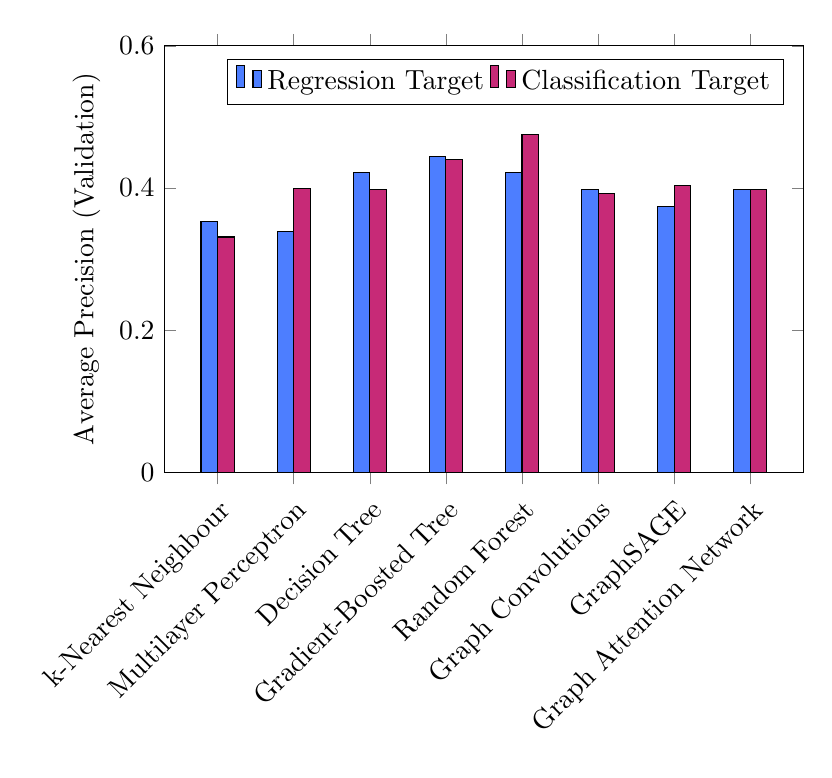
\begin{tikzpicture}
\definecolor{plotBlue}{RGB}{77,126,255}
\definecolor{plotPurple}{RGB}{97,75,202}
\definecolor{plotViolet}{RGB}{199,42,119}
\definecolor{plotOrange}{RGB}{245,80,27}
\definecolor{plotGreen}{RGB}{105,208,134}
\definecolor{plotBlack}{RGB}{255,255,255}
    \begin{axis}[
    ybar,
    bar width=6pt,
    width=0.8\textwidth,
    height=7cm,
    ymin=0,
    ymax=0.6,
    ylabel={Average Precision (Validation)},
    xtick=data,
    symbolic x coords={
        k-Nearest Neighbour,
        Multilayer Perceptron,
        Decision Tree,
        Gradient-Boosted Tree,
        Random Forest,
        Graph Convolutions,
        GraphSAGE,
        Graph Attention Network,
    },
    xticklabel style={rotate=45,anchor=north east},
    legend style={
        legend pos=north east,
        legend columns=2
    },
    ]

    \addplot[bar shift=-3pt,fill=plotBlue] coordinates {
        (Gradient-Boosted Tree, 0.4440352880707719)
        (Random Forest, 0.42126508450262135)
        (Decision Tree, 0.42126508450262135)
        (k-Nearest Neighbour, 0.3523807949098656)
        (Multilayer Perceptron, 0.33911571818438374)
        (Graph Convolutions, 0.3973)
        (GraphSAGE, 0.3734)
        (Graph Attention Network, 0.3973)
    };
    \addplot[bar shift=3pt,fill=plotViolet] coordinates {
        (Gradient-Boosted Tree, 0.44070016250479127)
        (Random Forest, 0.4747743632481278)
        (Decision Tree, 0.3983861433611597)
        (k-Nearest Neighbour, 0.3311685029371058)
        (Multilayer Perceptron, 0.39983671017473515)
        (Graph Convolutions, 0.3921)
        (GraphSAGE, 0.4030)
        (Graph Attention Network, 0.3984)
    };
    \legend{Regression Target,Classification Target}
    
    \end{axis}
\end{tikzpicture}
\caption{
    Average precision values of different models on validation data when classifying theories as problematic,
    for both regression (for lint frequency) and classification training targets.
}\label{fig:lint_freq_models_comp}
\end{figure}
It is evident that the deep learning models
do not perform better than classical models on our dataset,
which is not uncommon for data with noise in the ground truth
(of which we would expect quite a lot given the scenario).
Overall, the random forest model trained as a classifier is the best model with a validation AP of $0.47$.
Its precision-recall curve on the test data is shown in Figure~\ref{fig:rf_prc}.
\input{figures/rf_prc}
With a test AP of $0.51$, the model generalizes quite well---%
for example, \SI{58}{\percent} precision and \SI{21}{\percent} recall can be reached at a default threshold of $0.5$,
and the model is far better than random on the whole range.
This shows that while lints cannot be predicted very accurately,
they do reflect strongly on the formal entity graphs.

To find out which features are most important,
we perform an ablation study with the random forest model,
i.e., we iteratively re-train the model, removing the feature that leads to the smallest decrease in validation AP\@.
Figure~\ref{fig:lint_freq_rf_feats} shows the result.
\begin{figure}
\centering
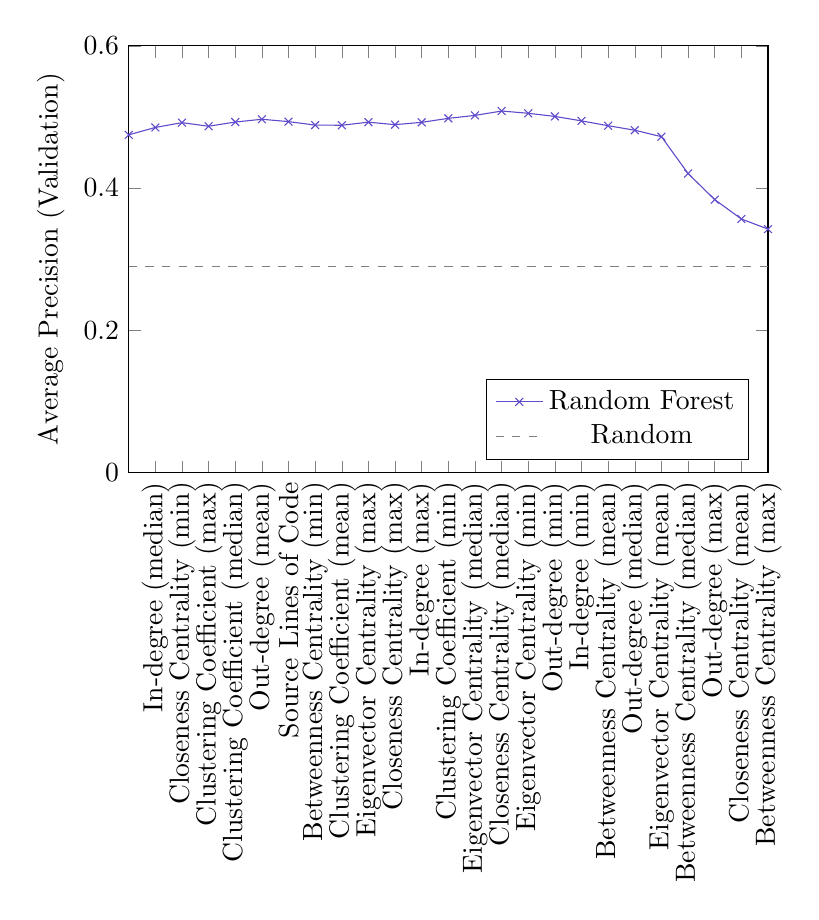
\begin{tikzpicture}
\definecolor{plotBlue}{RGB}{77,126,255}
\definecolor{plotPurple}{RGB}{97,75,202}
\definecolor{plotViolet}{RGB}{199,42,119}
\definecolor{plotOrange}{RGB}{245,80,27}
\definecolor{plotGreen}{RGB}{105,208,134}
\definecolor{plotBlack}{RGB}{0,0,0}
    \begin{axis}[
    width=0.8\textwidth,
    height=7cm,
    xlabel={},
    ylabel={Average Precision (Validation)},
    xtick=data,
    ymin=0,
    ymax=0.6,
    symbolic x coords={
\empty,
In-degree (median),
Closeness Centrality (min),
Clustering Coefficient (max),
Clustering Coefficient (median),
Out-degree (mean),
Source Lines of Code,
Betweenness Centrality (min),
Clustering Coefficient (mean),
Eigenvector Centrality (max),
Closeness Centrality (max),
In-degree (max),
Clustering Coefficient (min),
Eigenvector Centrality (median),
Closeness Centrality (median),
Eigenvector Centrality (min),
Out-degree (min),
In-degree (min),
Betweenness Centrality (mean),
Out-degree (median),
Eigenvector Centrality (mean),
Betweenness Centrality (median),
Out-degree (max),
Closeness Centrality (mean),
Betweenness Centrality (max),
    },
    xticklabel style={rotate=90},
    xmin=\empty,
    xmax=Betweenness Centrality (max),
    legend pos=south east,
    ]
    \addplot[color=plotPurple,mark=x] coordinates {
(\empty,0.4748)
(In-degree (median),0.4852)
(Closeness Centrality (min),0.4919)
(Clustering Coefficient (max),0.4869)
(Clustering Coefficient (median),0.4928)
(Out-degree (mean),0.4967)
(Source Lines of Code,0.4934)
(Betweenness Centrality (min),0.4885)
(Clustering Coefficient (mean),0.4883)
(Eigenvector Centrality (max),0.4926)
(Closeness Centrality (max),0.4891)
(In-degree (max),0.4924)
(Clustering Coefficient (min),0.4980)
(Eigenvector Centrality (median),0.5021)
(Closeness Centrality (median),0.5083)
(Eigenvector Centrality (min),0.5051)
(Out-degree (min),0.5007)
(In-degree (min),0.4944)
(Betweenness Centrality (mean),0.4876)
(Out-degree (median),0.4813)
(Eigenvector Centrality (mean),0.4722)
(Betweenness Centrality (median),0.4204)
(Out-degree (max),0.3837)
(Closeness Centrality (mean),0.3565)
(Betweenness Centrality (max),0.3422)
    };

    \addplot[mark=none,dashed,color=gray] coordinates {
        (\empty,0.29) (Betweenness Centrality (max),0.29)
    };
    \legend{Random Forest,Random};
    \end{axis}
\end{tikzpicture}
\caption{
    Average precision for best random forest model after tuning,
    when cumulatively removing features.
    In-degree (mean) remains as last feature.
}\label{fig:lint_freq_rf_feats}
\end{figure}
Initially, the score fluctuates slightly,
until it eventually takes a steep decline---%
at the turning point,
betweenness centrality (median and max), out-degree (max), closeness centrality (mean), and in-degree (mean),
remain.

\subsection{Comparison with Perceived Quality}\label{sec:llama}
Obtaining a dataset for perceived quality is quite difficult,
since often only domain experts are capable of judging the quality of a given formalization,
especially when it comes to quality problems that are not obvious.
By inquiring Isabelle experts in various domains about theories or AFP developments they would consider good and bad quality,
we obtained a ground-truth sample of $70$ labelled theories
($35$ good and bad each).
Importantly,
we did not give a definition of quality
(relying on the experts' intuition)
nor did we contribute any data ourselves,
so as not to skew the dataset in any way.
As an example,
one expert classified a theory as problematic because the assumptions on the main theorem were stronger than needed,
making it unusable to them.

While $70$ examples is not enough data to train any models on,
the sample is sufficiently large to evaluate both the lint results and our other machine learning model discussed previously.
In addition,
we evaluate the un-tuned capabilities of a large language model:
By prompting the pre-trained LLAMA ($7$ billion parameters) transformer~\cite{touvron2023llama}
about the quality of chunks of formalization code
(on a scale from $1$ to $10$)
and averaging the scores for each theory,
we obtained quality predictions for the whole AFP\@.
Even though we did not fine-tune the model due to the prohibitive hardware requirements,
its responses sound mostly coherent, e.g., a score of $2$ was given with the justification that \enquote{the lemma \texttt{equivclp\_least[OF hash]} is a bit cryptic and I would prefer something more explicit and readable}.

With our pre-defined threshold of one lint every $100$ lines,
we achieved \SI{95}{\percent} precision and \SI{51}{\percent} recall
at predicting bad-quality theories on our sample,
whereas the random forest model scored \SI{43}{\percent} precision and \SI{100}{\percent} recall.
\begin{figure}
\centering
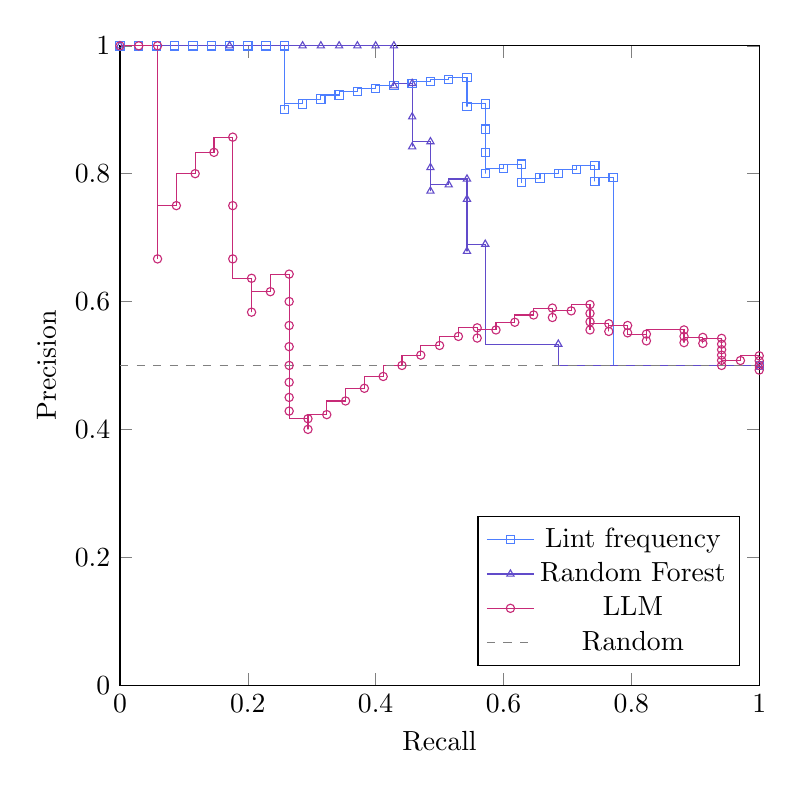
\begin{tikzpicture}
\definecolor{plotBlue}{RGB}{77,126,255}
\definecolor{plotPurple}{RGB}{97,75,202}
\definecolor{plotViolet}{RGB}{199,42,119}
\definecolor{plotOrange}{RGB}{245,80,27}
\definecolor{plotGreen}{RGB}{105,208,134}
\definecolor{plotBlack}{RGB}{0,0,0}
    \begin{axis}[
        xlabel={Recall},
        ylabel={Precision},
        xmin=0, xmax=1,
        ymin=0, ymax=1,
        grid=none,
        width=0.8\textwidth,
        height=0.8\textwidth,
        legend pos=south east,
    ]

        \addplot[const plot mark left,mark=square,mark size=1.5pt,color=plotBlue] coordinates {
(1.00000000,0.50000000) (0.77142857,0.79411765) (0.74285714,0.78787879) (0.74285714,0.81250000) (0.71428571,0.80645161) (0.68571429,0.80000000) (0.65714286,0.79310345) (0.62857143,0.78571429) (0.62857143,0.81481481) (0.60000000,0.80769231) (0.57142857,0.80000000) (0.57142857,0.83333333) (0.57142857,0.86956522) (0.57142857,0.90909091) (0.54285714,0.90476190) (0.54285714,0.95000000) (0.51428571,0.94736842) (0.48571429,0.94444444) (0.45714286,0.94117647) (0.42857143,0.93750000) (0.40000000,0.93333333) (0.37142857,0.92857143) (0.34285714,0.92307692) (0.31428571,0.91666667) (0.28571429,0.90909091) (0.25714286,0.90000000) (0.25714286,1.00000000) (0.22857143,1.00000000) (0.20000000,1.00000000) (0.17142857,1.00000000) (0.14285714,1.00000000) (0.11428571,1.00000000) (0.08571429,1.00000000) (0.05714286,1.00000000) (0.02857143,1.00000000) (0.00000000,1.00000000)
        };
        \addplot[const plot mark left,mark=triangle,mark size=1.5pt,color=plotPurple] coordinates {
(1.00000000,0.50000000) (0.68571429,0.53333333) (0.57142857,0.68965517) (0.54285714,0.67857143) (0.54285714,0.76000000) (0.54285714,0.79166667) (0.51428571,0.78260870) (0.48571429,0.77272727) (0.48571429,0.80952381) (0.48571429,0.85000000) (0.45714286,0.84210526) (0.45714286,0.88888889) (0.45714286,0.94117647) (0.42857143,0.93750000) (0.42857143,1.00000000) (0.40000000,1.00000000) (0.37142857,1.00000000) (0.34285714,1.00000000) (0.31428571,1.00000000) (0.28571429,1.00000000) (0.17142857,1.00000000) (0.00000000,1.00000000)
        };
        \addplot[const plot mark left,mark=o,mark size=1.5pt,color=plotViolet] coordinates {
(1.00000000,0.49275362) (1.00000000,0.50000000) (1.00000000,0.50746269) (1.00000000,0.51515152) (0.97058824,0.50769231) (0.94117647,0.50000000) (0.94117647,0.50793651) (0.94117647,0.51612903) (0.94117647,0.52459016) (0.94117647,0.53333333) (0.94117647,0.54237288) (0.91176471,0.53448276) (0.91176471,0.54385965) (0.88235294,0.53571429) (0.88235294,0.54545455) (0.88235294,0.55555556) (0.82352941,0.53846154) (0.82352941,0.54901961) (0.79411765,0.55102041) (0.79411765,0.56250000) (0.76470588,0.55319149) (0.76470588,0.56521739) (0.73529412,0.55555556) (0.73529412,0.56818182) (0.73529412,0.58139535) (0.73529412,0.59523810) (0.70588235,0.58536585) (0.67647059,0.57500000) (0.67647059,0.58974359) (0.64705882,0.57894737) (0.61764706,0.56756757) (0.58823529,0.55555556) (0.55882353,0.54285714) (0.55882353,0.55882353) (0.52941176,0.54545455) (0.50000000,0.53125000) (0.47058824,0.51612903) (0.44117647,0.50000000) (0.41176471,0.48275862) (0.38235294,0.46428571) (0.35294118,0.44444444) (0.32352941,0.42307692) (0.29411765,0.40000000) (0.29411765,0.41666667) (0.26470588,0.42857143) (0.26470588,0.45000000) (0.26470588,0.47368421) (0.26470588,0.50000000) (0.26470588,0.52941176) (0.26470588,0.56250000) (0.26470588,0.60000000) (0.26470588,0.64285714) (0.23529412,0.61538462) (0.20588235,0.58333333) (0.20588235,0.63636364) (0.17647059,0.66666667) (0.17647059,0.75000000) (0.17647059,0.85714286) (0.14705882,0.83333333) (0.11764706,0.80000000) (0.08823529,0.75000000) (0.05882353,0.66666667) (0.05882353,1.00000000) (0.02941176,1.00000000) (0.00000000,1.00000000)
        };

        \addplot[mark=none,color=gray,dashed] coordinates {
            (0,0.5) (1,0.5)
        };

        \legend{Lint frequency,Random Forest,LLM,Random}

    \end{axis}
\end{tikzpicture}
\caption{Precision-recall curves on ground truth data set for different models.}\label{fig:ground_prcs}
\end{figure}
Figure~\ref{fig:ground_prcs} shows the full precision-recall curves for our three classifiers.
The lint frequency remains an excellent estimator even for high thresholds where recall goes up to \SI{77}{\percent} (at \SI{79}{\percent} precision),
and is outperformed by the random forest model only in the low-recall regions
(where the latter attains perfect precision for up to \SI{43}{\percent} recall).
The large language model performs well in the low-recall regions,
which is surprising given that it has not been trained on Isabelle quality at all,
suggesting that textual structure alone
(which is what the model understands)
can give a hint about overall quality.
However, for higher thresholds,
it is close to random.
